\documentclass{beamer}
\usepackage[british,spanish]{babel}
\usepackage[utf8]{inputenc}
\usepackage{hyperref}
\usepackage{multirow}

\usepackage{listings}

\usepackage{adjustbox}
\usepackage{lstcustom}

\usepackage{color}
\definecolor{light-gray}{gray}{0.80}
\definecolor{lstbackgroundshellcolor}{named}{light-gray}

\usepackage{tikz}
\newcommand*\circled[1]{\tikz[baseline=(char.base)]{
            \node[shape=circle,draw,inner sep=2pt] (char) {#1};}}

\usepackage[normalem]{ulem}

\newcommand{\comment}[2]{#2}


\title[Learning Android]{Learning Android}
%\subtitle[short subtitle]{long subtitle}
\author[C. Cuenca]{Carmelo Cuenca-Hernández}
%\institute{Escuela Universitaria de Informática}
%\date[04/2013]{Abril - 2013}
\date{}
\titlegraphic{\includegraphics[width=0.5 \textwidth]{logo_ulpgc_version_horizontal_rgb.eps}}



\pgfdeclareimage[width=2.0\baselineskip]{ulpgc-logo}{logosimbolo_secundario_version_vertical}
\setbeamertemplate{footline}{\raisebox{-2ex}{\pgfuseimage{ulpgc-logo}}
  \usebeamerfont{date in head/foot}\insertshortdate{}\hfill
  \usebeamertemplate{navigation symbols}\hfill
  \insertframenumber{}/\inserttotalframenumber}
\setbeamertemplate{sidebar right}{}


\usetheme{Antibes}
%\usetheme{Berlin}

%\usetheme{Warsaw}
%\usecolortheme{albatross}

\begin{document}

\begin{frame}
	\titlepage
\end{frame}


\section*{Outline}
\begin{frame}
	\frametitle{Outline}
	%\tableofcontents%[part=1,pausesections]
%\tableofcontents[currentsection,currentsubsection, sectionstyle=show] 
\tableofcontents[currentsection,sectionstyle=show,hideothersubsections]
\end{frame}


\selectlanguage{british}



%%%%%%%%%%%%%%%%%%%%%%%%%%%%%%%%%%%%%%%%%%%%%%%%%%%%%%%%%%%%%%%%%%%%%%%%%%%%%%%%%
\section{Android Overview}
%%%%%%%%%%%%%%%%%%%%%%%%%%%%%%%%%%%%%%%%%%%%%%%%%%%%%%%%%%%%%%%%%%%%%%%%%%%%%%%%
%------------------------------------------------------------------------------
\begin{frame}
\frametitle{Android Overview}
\alert{Android} is a comprehensive open source platform designed for mobile devices. It is championed by Google and owned by \href{http://www.openhandsetalliance.com/}{Open Handset Alliance}.
\begin{description}
	\item[Comprehensive] The Android SDK is all you need to start developing for Android.
	\item[Open Source Platform] Android is licensed under business-friendly licenses (Apache/MIT).
\end{description}
\end{frame}
%------------------------------------------------------------------------------
\subsection{History}
\begin{frame}
\frametitle{History}
\begin{enumerate}
	\item In 2005, Google buys Android Inc.
	\item In 2007, the Open Handset Alliance is announced.
	\item In 2008, the Android SDK 1.0 is released. The G1 phone, manufactured by HTC.
	\item 2009 sees a proliferation of Android-based devices. More than 20 devices run Android.
	\item In 2010, Android is second only to Blackberry as the best-selling smart phone platform. More than 60 devices that run Froyo.
\end{enumerate}
\end{frame}

%------------------------------------------------------------------------------
\subsection{Android Versions}
\begin{frame}
\frametitle{Android Versions}
\begin{table}[h]
\begin{tabular}{|c|c|c|c|} \hline
\multicolumn{4}{|c|}{\href{http://developer.android.com/about/dashboards/index.html}{Android Device Dashboard from 2013}} \\ \hline
Version & Codename &	API &	Distribution \\ \hline
1.6 & Donut & 4	& 0.2\% \\ \hline
2.1 & Eclair & 7 & 1.9\% \\ \hline
2.2 & Froyo  & 8 & 7.5\% \\ \hline
2.3 - 2.3.2 & \multirow{2}{*}{Gingerbread} & 9 &0.2\% \\
2.3.3 - 2.3.7 & & 10 & 43.9\% \\ \hline
3.1 & \multirow{2}{*}{Honeycomb} & 12 & 0.3\% \\
3.2 & & 13 & 0.9\% \\ \hline
4.0.3 - 4.0.4 & Ice Cream Sandwich & 15	& 28.6\% \\ \hline
4.1 & \multirow{2}{*}{Jelly Bean} & 16 & 14.9\% \\
4.2 & & 17 & 1.6\% \\ \hline
\end{tabular}
\caption{Data collected during a 14-day period ending on March 4, 2013.}
\end{table}
\end{frame}

%------------------------------------------------------------------------------
\subsection{The Stack}
\begin{frame}
\frametitle{The Stack}
\centering
\begin{columns}
\column{0.70\textwidth}
\centering
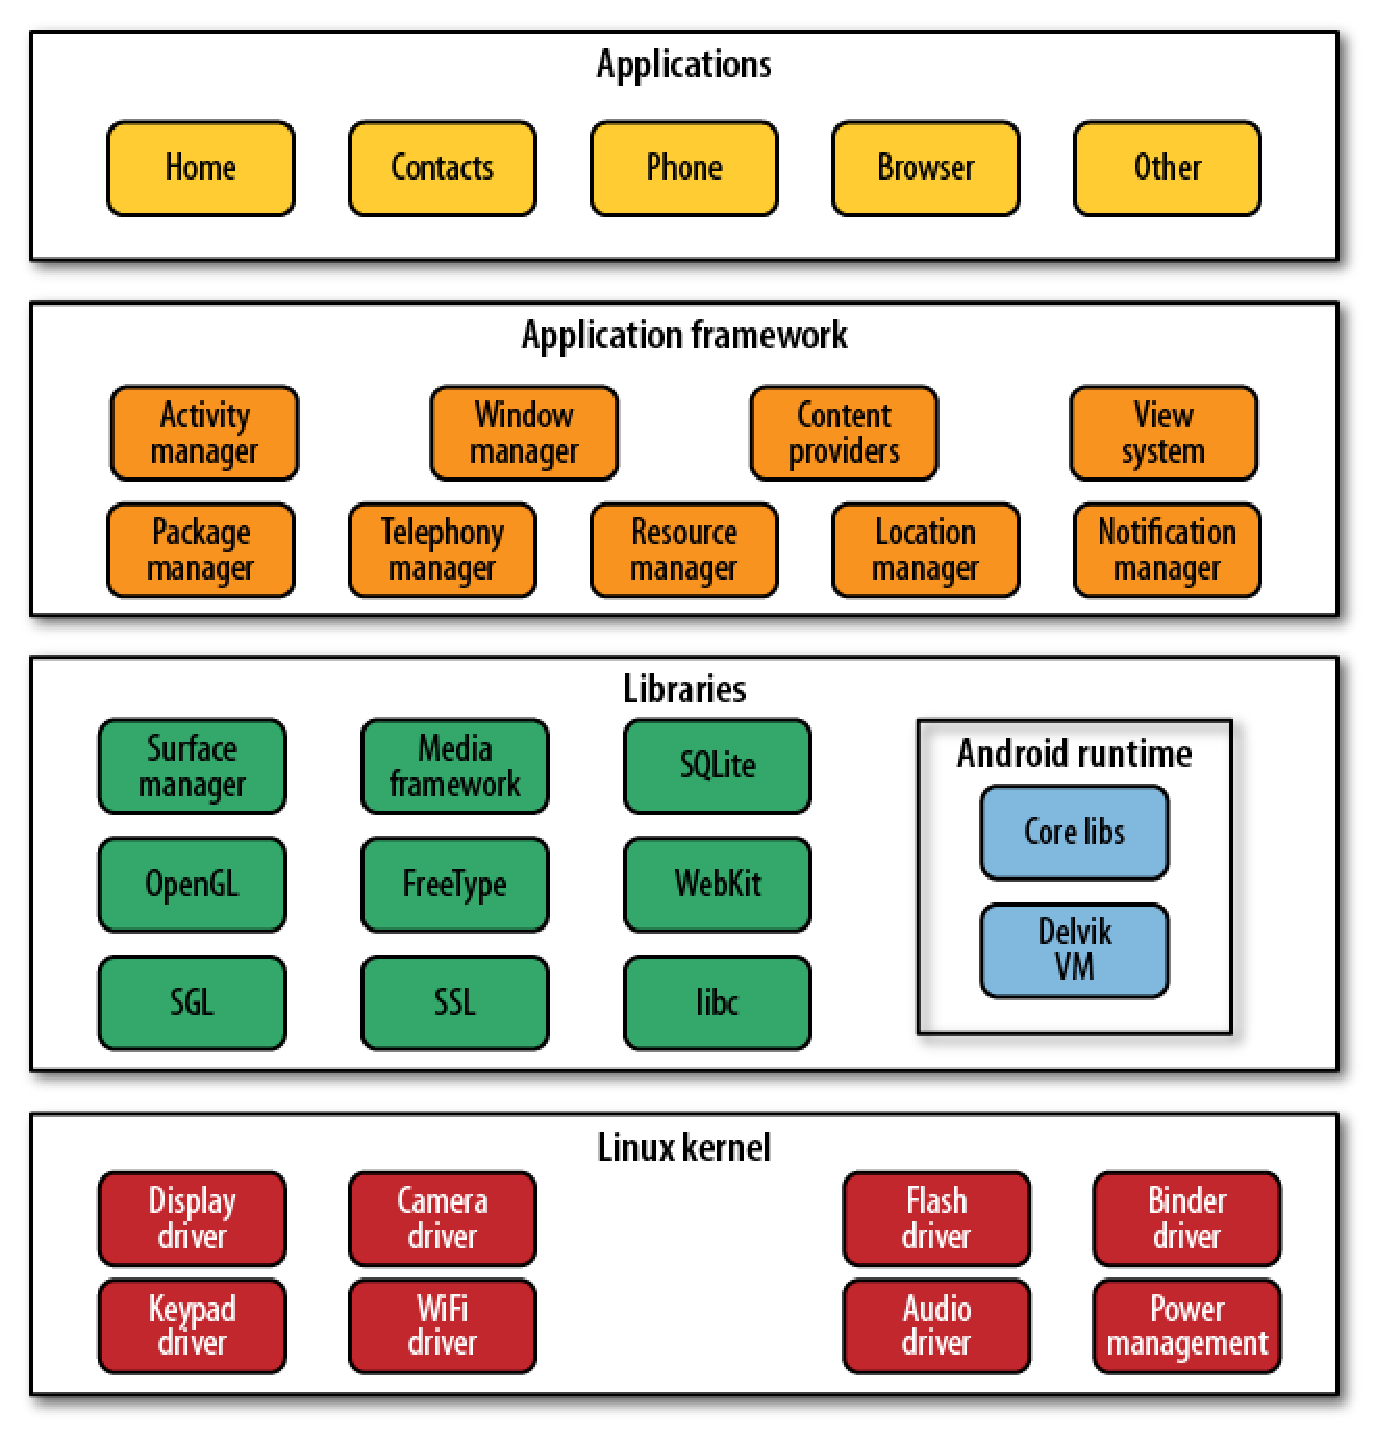
\includegraphics[width= 0.60 \textwidth]{fig-7.eps}
\column{0.45 \textwidth}
\begin{itemize}
\item Linux
\item Native Libraries
\item Dalvik
\item Application Framework
\item Applications
\end{itemize}


\end{columns}
\end{frame}

%------------------------------------------------------------------------------
\begin{frame}
\frametitle{Linux}
Android is built on top of \alert{Linux}.
\begin{description}
	\item[Portability] Linux is a portable platform that is relatively easy to compile on various hardware architectures
	\item[Security] All Android applications run as separate Linux processes with permissions set by the Linux system
	\item[Features] Memory management, power management, and networking
\end{description}
\end{frame}
%------------------------------------------------------------------------------
\begin{frame}
\frametitle{Native Libraries}
The \alert{native libraries} are C/C++ libraries, often taken from the open source community
in order to provide necessary services to the Android application layer. Among others,
they include:
\begin{description}
	\item[Webkit] A fast web-rendering engine used by Safari, Chrome, and other browsers
	\item[SQLite] A full-featured SQL database
	\item[Apache Harmony] An open source implementation of Java
	\item[OpenGL] 3D graphics libraries
	\item[OpenSSL] The secure locket layer
	\item[Bionic] A rewritten version of the standard C library
\end{description}
\end{frame}
%------------------------------------------------------------------------------
\begin{frame}
\frametitle{Dalvik, Android and  Java}
\alert{Dalvik} is a purpose-built virtual machine designed specifically for Android, developed
by Dan Bornstein and his team at Google
\centering
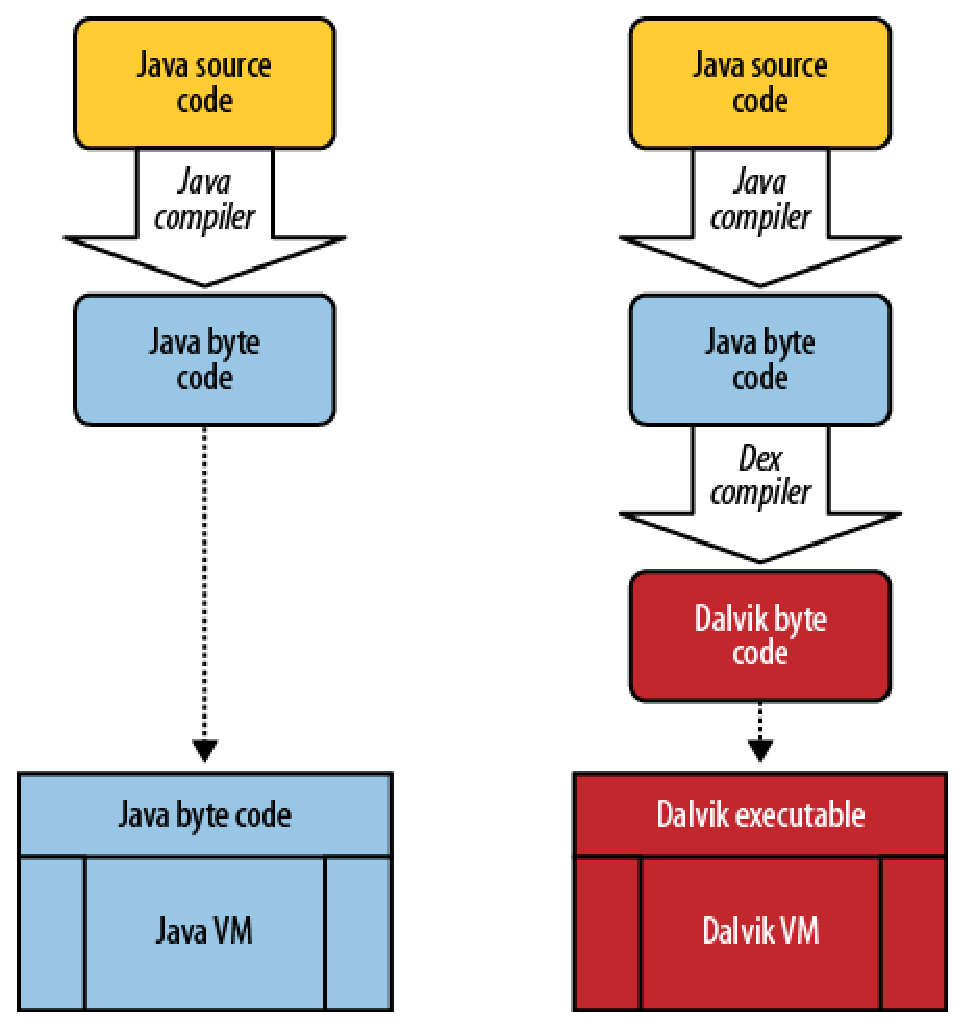
\includegraphics[width= 0.40 \linewidth]{fig-9.eps}
\end{frame}
%------------------------------------------------------------------------------
\begin{frame}
\frametitle{Application Framework}
The \alert{application framework} is a rich environment that provides numerous services to
help you, the app developer, get your job done
\begin{columns}
\column{0.65 \textwidth}
\centering
\includegraphics[width= 1.0 \textwidth]{fig-2001.eps}
\end{columns}
\end{frame}
%------------------------------------------------------------------------------
\begin{frame}
\frametitle{Applications}
An \alert{application} is a single application package (APK) file. An APK file roughly has three
main components:
\begin{description}
	\item[Dalvik executable] Java source code compiled down to a Dalvik executable
	\item[Resources] Resources are everything that is not code (images, audio/video clips, XML files describing layouts, language packs \dots
	\item[Native libraries] Your application may include some native code, such as C/C++ libraries
\end{description}
\end{frame}
%------------------------------------------------------------------------------
\subsection[Plattform Set Up]{Plattform Set Up}
\begin{frame}
\frametitle{Plattform Set Up}
\begin{enumerate}
 	\item Install the Android SDK, \href{http://developer.android.com/sdk/index.html}{Android SDK Download page}
	\item Install the Platform-tools, using the SDK Manager \texttt{tools/android update sdk --no-ui}
	\item Install Eclipse, \href{http://www.eclipse.org/downloads}{Eclipse IDE for Java Developers}
	\item Instal Android Tool for Eclipse (Android DDMS and Android Development Tools), \url{https://dl-ssl.google.com/android/}

\end{enumerate}
\end{frame}
%------------------------------------------------------------------------------
\subsection{Hello World!}

%------------------------------------------------------------------------------
\begin{frame}
\frametitle{Hello Wolrd!}
\begin{columns}
\column{0.5 \textwidth}
\centering
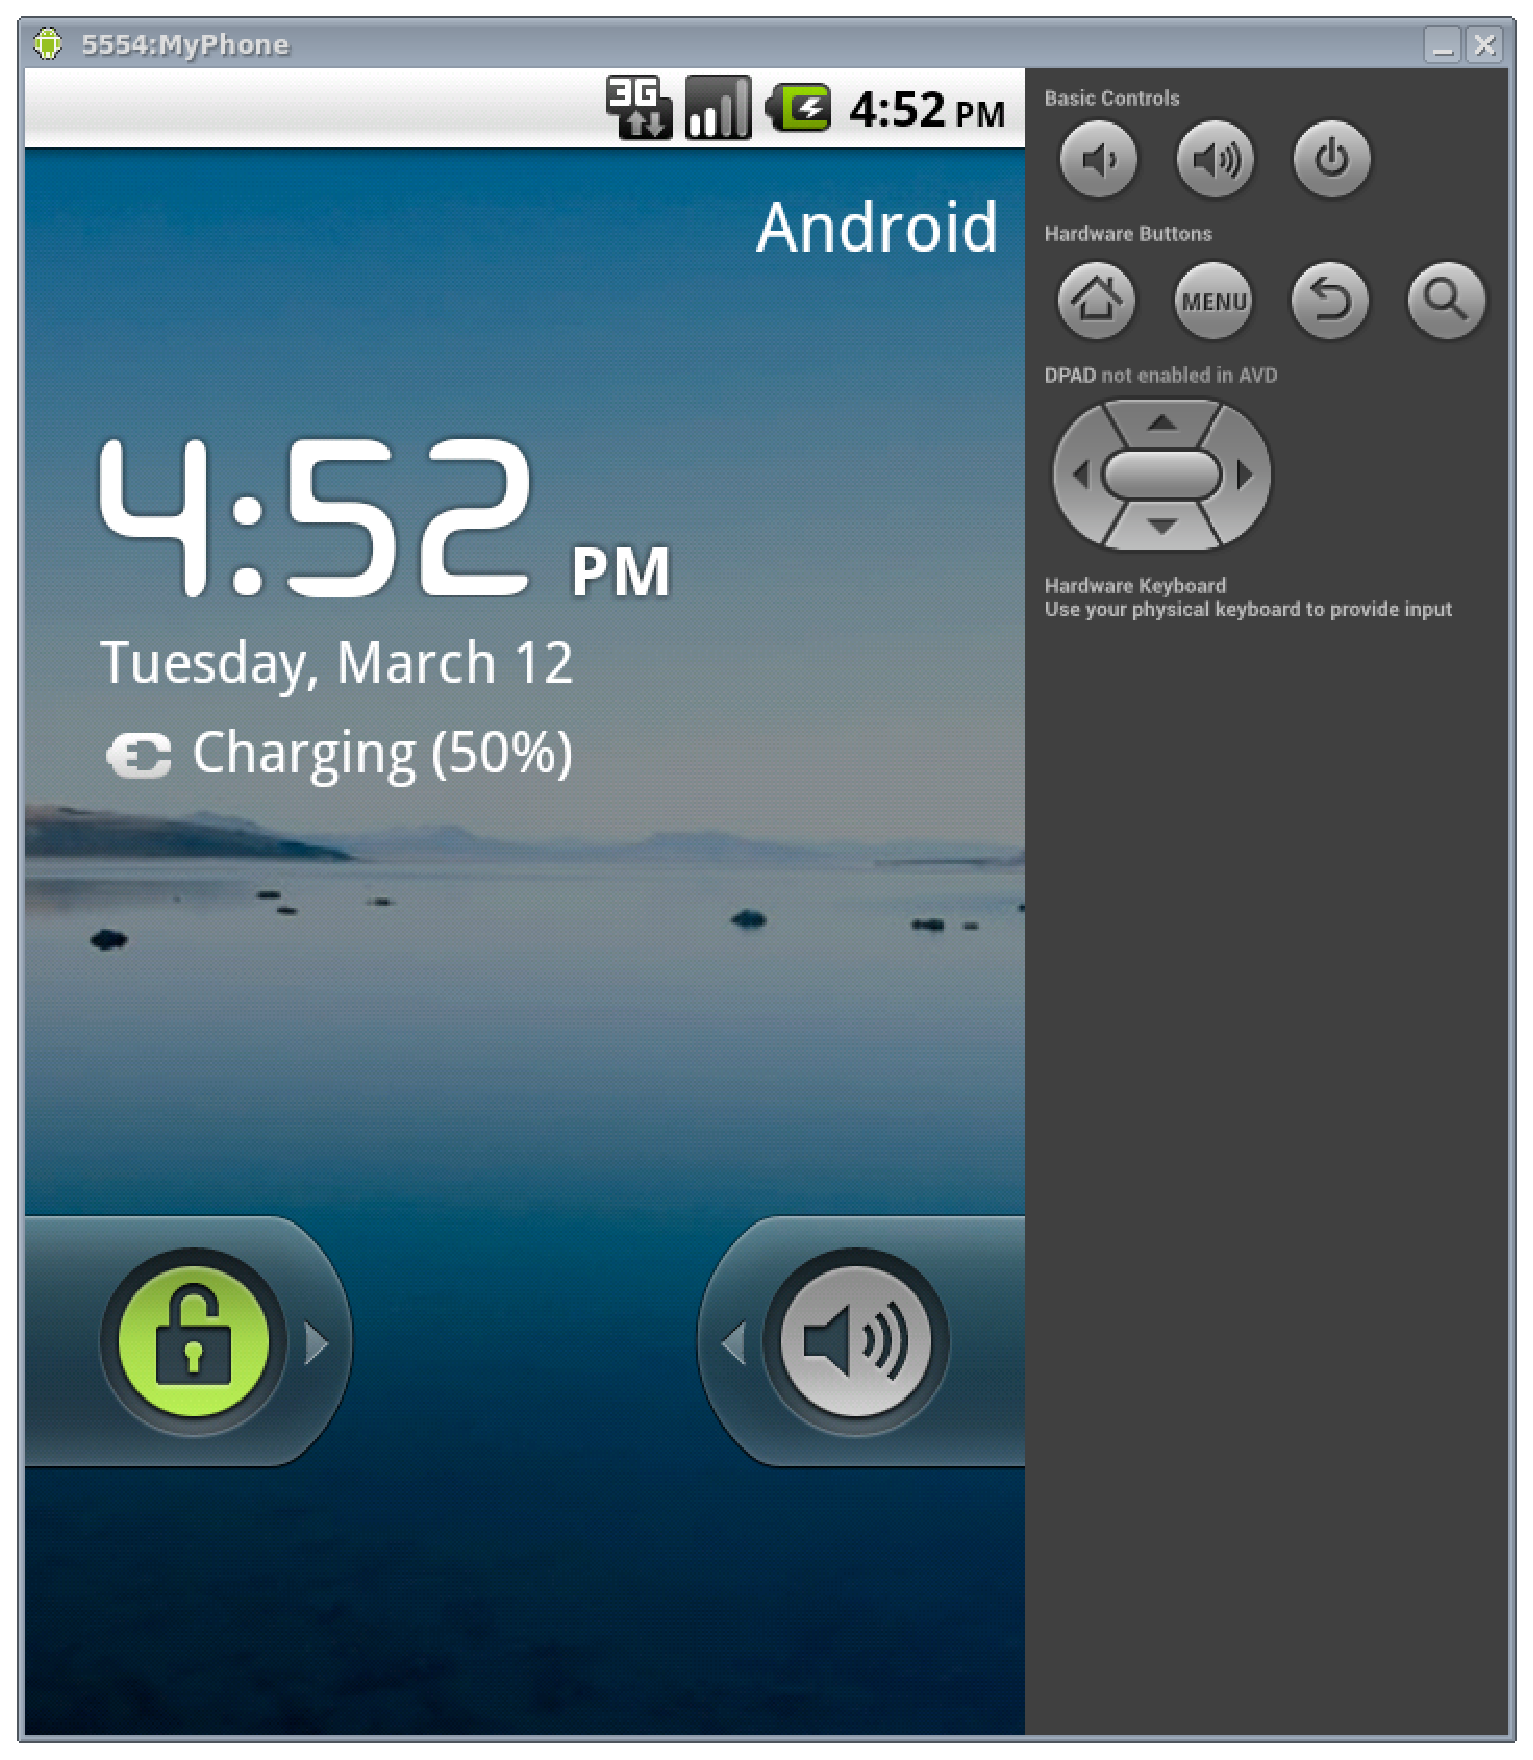
\includegraphics[width= 1.0 \textwidth]{MyPhone.eps}
\column{0.5 \textwidth}
\centering
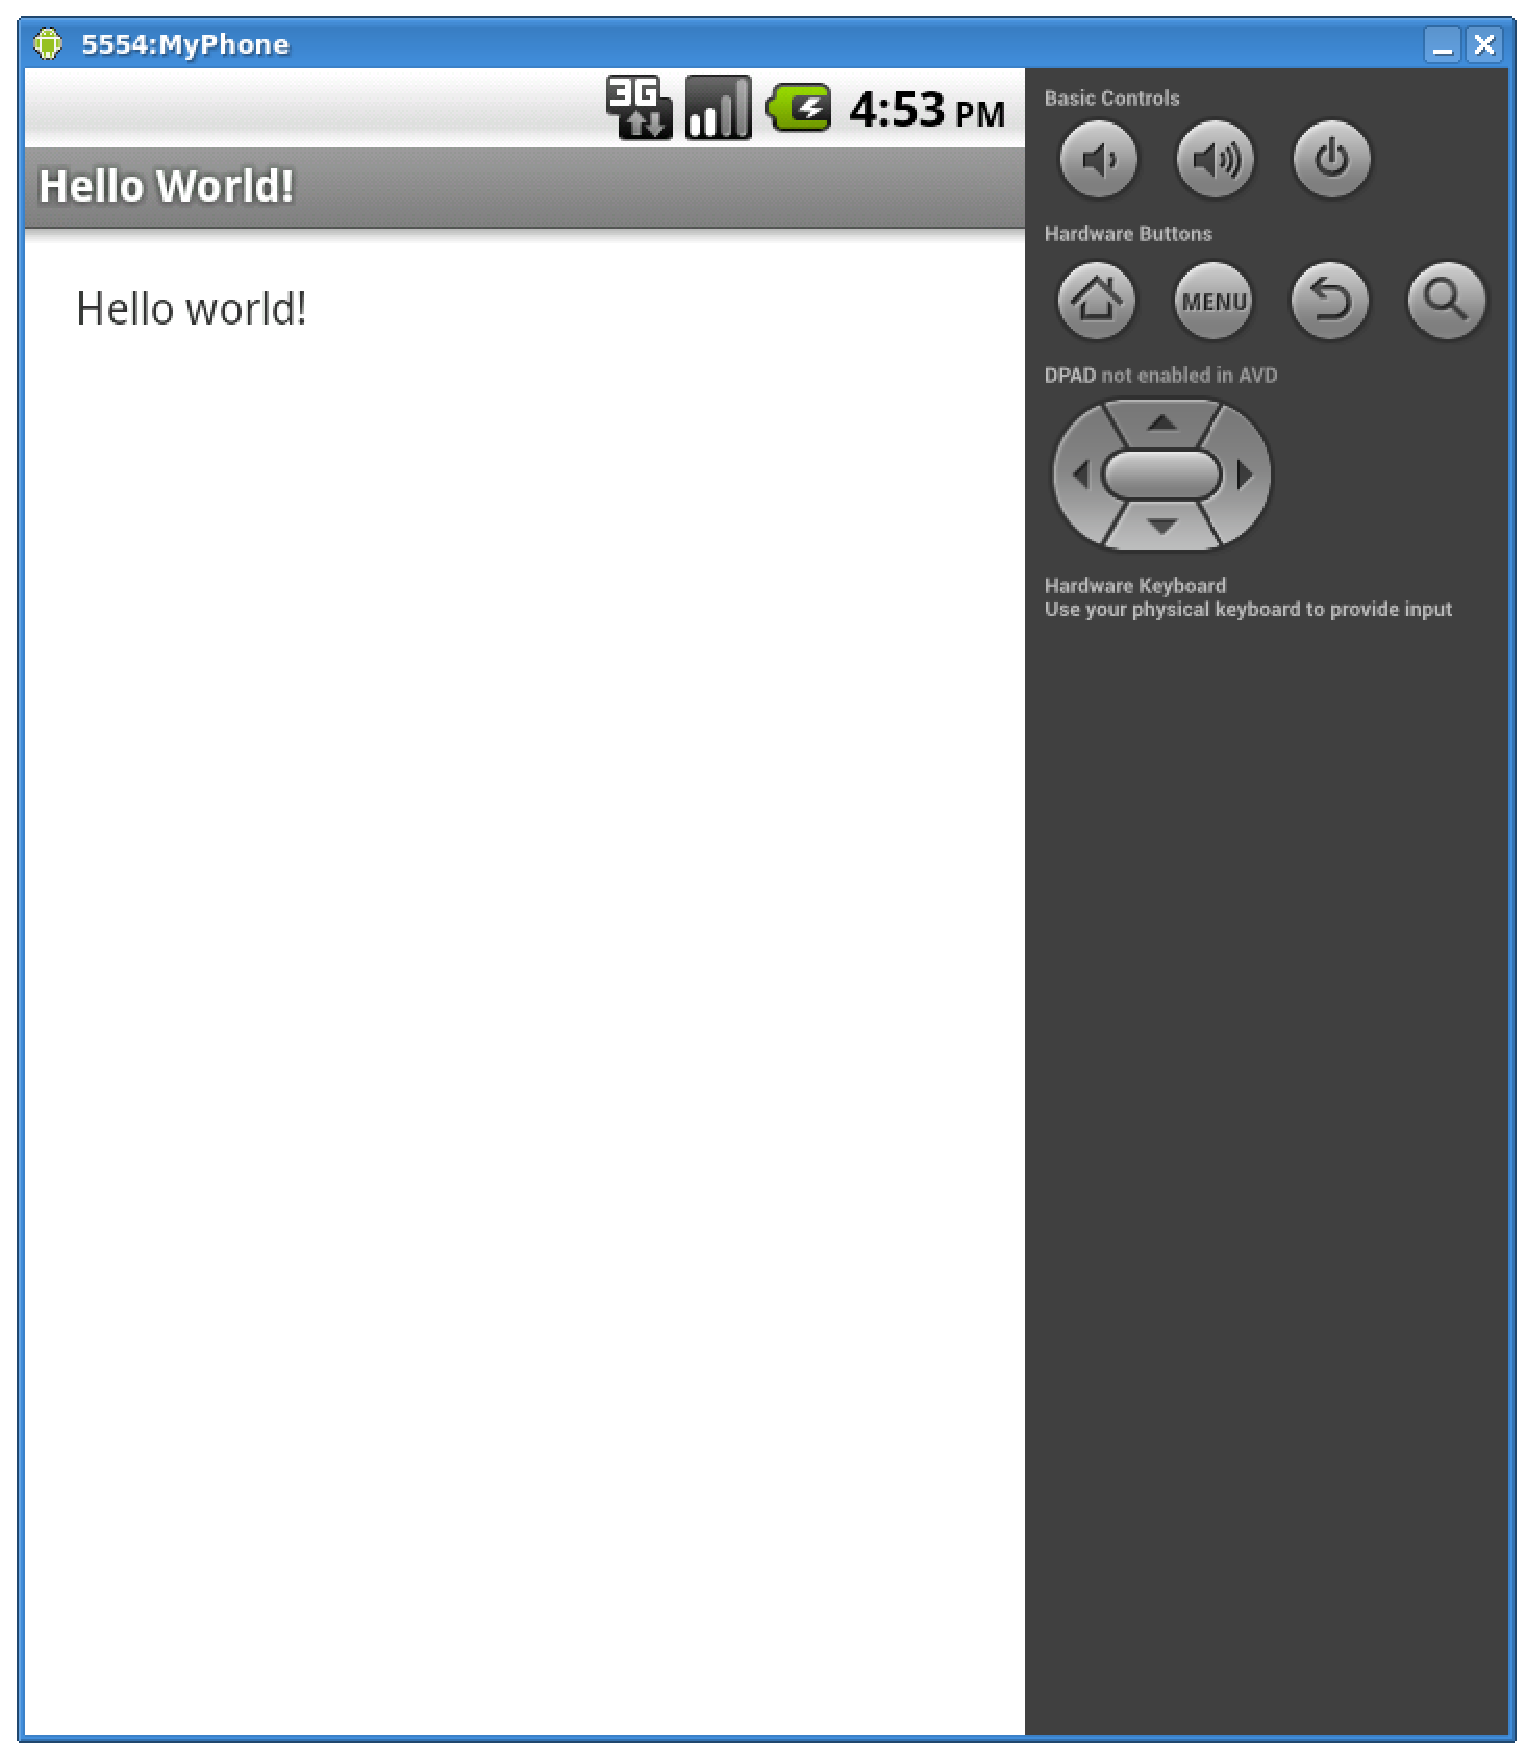
\includegraphics[width= 1.0 \textwidth]{HelloWorld.eps}
\end{columns}
\end{frame}
%------------------------------------------------------------------------------

\begin{frame}
\frametitle{Creating a New Project}
\textbf{File|New Android Application Project}\\
\alert{Application Name}, \alert{Project Name}, \alert{Package Name}

\begin{columns}
\column{0.45 \textwidth}
\centering
\includegraphics[width= 1.0 \textwidth]{NewAndroidApplication1.eps}
\column{0.65 \textwidth}
\begin{description}
 	\item[Application Name] \textbf{Hello World!} The application name is the plain English name of your application
	\item[Project Name] \textbf{HelloWorld} Eclipse organizes everything into projects. A project name should be one word
	\item[Package Name] \textbf{com.artemisa} In Java, all source code is organized into packages
\end{description}
\end{columns}
\end{frame}
%------------------------------------------------------------------------------
\begin{frame}[fragile]
\frametitle{Manifiest File}
The manifest file explains what the application consists of
\lstset{language=XML, style=eclipse}
\begin{adjustbox}{width=0.8 \textwidth}
\begin{lstlisting}[caption=AndroidManifiest.xml]
<?xml version="1.0" encoding="utf-8"?>
<manifest xmlns:android="http://schemas.android.com/apk/res/android"
    package="com.artemisa.helloworld"
    android:versionCode="1"
    android:versionName="1.0" >

    <uses-sdk
        android:minSdkVersion="8"
        android:targetSdkVersion="17" />

    <application
        android:allowBackup="true"
        android:icon="@drawable/ic_launcher"
        android:label="@string/app_name"
        android:theme="@style/AppTheme" >
        <activity
            android:name="com.artemisa.helloworld.MainActivity"
            android:label="@string/app_name" >
            <intent-filter>
                <action android:name="android.intent.action.MAIN" />

                <category android:name="android.intent.category.LAUNCHER" />
            </intent-filter>
        </activity>
    </application>

</manifest>
\end{lstlisting}
\end{adjustbox}
\end{frame}
%------------------------------------------------------------------------------
\begin{frame}[fragile]
\frametitle{Layout XML Code}
The layout file specifies the layout of your screen. Layout XML is responsible for the layout of widgets
\lstset{language=XML, style=eclipse}
\begin{adjustbox}{width=1.0 \textwidth}
\begin{lstlisting}[caption=res/layout/activity\_main.xml]
<RelativeLayout xmlns:android="http://schemas.android.com/apk/res/android"
    xmlns:tools="http://schemas.android.com/tools"
    android:layout_width="match_parent"
    android:layout_height="match_parent"
    android:paddingBottom="@dimen/activity_vertical_margin"
    android:paddingLeft="@dimen/activity_horizontal_margin"
    android:paddingRight="@dimen/activity_horizontal_margin"
    android:paddingTop="@dimen/activity_vertical_margin"
    tools:context=".MainActivity" >

    <TextView
        android:layout_width="wrap_content"
        android:layout_height="wrap_content"
        android:text="@string/hello_world" />

</RelativeLayout>
\end{lstlisting}
\end{adjustbox}
\end{frame}
%------------------------------------------------------------------------------
\begin{frame}[fragile]
\frametitle{Strings}
This is another XML file that contains all the text that your application uses. Strings XML is responsible for their textual content
\lstset{language=XML, style=eclipse}
\begin{adjustbox}{width=1.0 \textwidth}
\begin{lstlisting}[caption=res/values/strings.xml]
<?xml version="1.0" encoding="utf-8"?>
<resources>

    <string name="app_name">Hello World!</string>
    <string name="action_settings">Settings</string>
    <string name="hello_world">Hello world!</string>

</resources>
\end{lstlisting}
\end{adjustbox}
\end{frame}
%------------------------------------------------------------------------------
\begin{frame}[fragile]
\frametitle{The R file}
The R file is the glue between Java and the resources
\lstset{language=java, style=eclipse, tabsize=2}
\begin{adjustbox}{width=0.5 \textwidth}
\begin{lstlisting}[caption=gen/artemisa/helloworld/R.java]
/* AUTO-GENERATED FILE.  DO NOT MODIFY.
 *
 * This class was automatically generated by the
 * aapt tool from the resource data it found.  It
 * should not be modified by hand.
 */

package com.artemisa.helloworld;

public final class R {
    public static final class attr {
    }
    public static final class dimen {
        /**  Default screen margins, per the Android Design guidelines. 

         Customize dimensions originally defined in res/values/dimens.xml (such as
         screen margins) for sw720dp devices (e.g. 10" tablets) in landscape here.
    
         */
        public static final int activity_horizontal_margin=0x7f040000;
        public static final int activity_vertical_margin=0x7f040001;
    }
    public static final class drawable {
        public static final int ic_launcher=0x7f020000;
    }
    public static final class id {
        public static final int action_settings=0x7f080000;
    }
    public static final class layout {
        public static final int activity_main=0x7f030000;
    }
    public static final class menu {
        public static final int main=0x7f070000;
    }
    public static final class string {
        public static final int action_settings=0x7f050001;
        public static final int app_name=0x7f050000;
        public static final int hello_world=0x7f050002;
    }
    // ...
}
\end{lstlisting}
\end{adjustbox}
\end{frame}
%------------------------------------------------------------------------------
\begin{frame}[fragile]
\frametitle{Java Source Code}
The Java code is what drives everything. This is the code that ultimately gets converted
to a Dalvik executable and runs your application
\lstset{language=java, style=eclipse, tabsize=2}
\begin{adjustbox}{width=0.85 \textwidth}
\begin{lstlisting}[caption=src/com/artemisa/helloworld/MainActivity.java]
package com.artemisa.helloworld;

import android.os.Bundle;
import android.app.Activity;
import android.view.Menu;

public class MainActivity extends Activity {

	@Override
	protected void onCreate(Bundle savedInstanceState) {
		super.onCreate(savedInstanceState);
		setContentView(R.layout.activity_main);
	}

	@Override
	public boolean onCreateOptionsMenu(Menu menu) {
		// Inflate the menu; this adds items to the action bar if it is present.
		getMenuInflater().inflate(R.menu.main, menu);
		return true;
	}

}
\end{lstlisting}
\end{adjustbox}
\end{frame}
%------------------------------------------------------------------------------
\begin{frame}
\frametitle{The Emulator}
To use the emulator, we’ll have to create an Android Virtual Device (AVD)
\begin{columns}
\column{1.0 \textwidth}
\centering
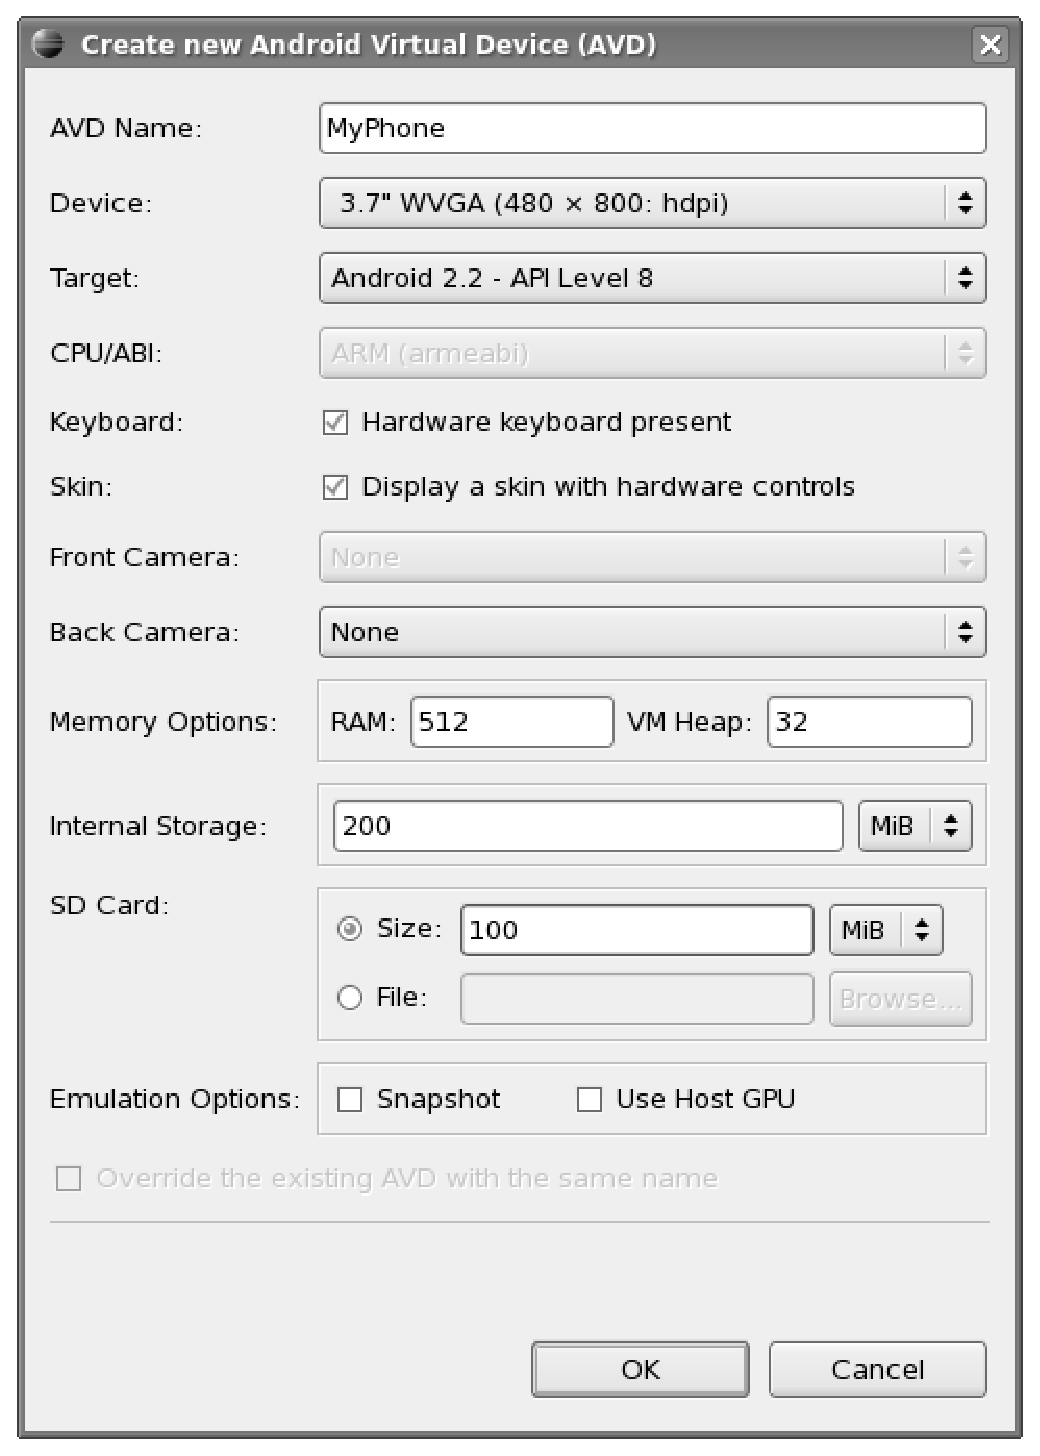
\includegraphics[width= 0.35 \textwidth]{CreateNewAndroidVitualDevice.eps}
\end{columns}
\end{frame}
%------------------------------------------------------------------------------
\begin{frame}
\frametitle{Go Ahead and Be Patient!}
\begin{columns}
\column{0.5 \textwidth}
\centering
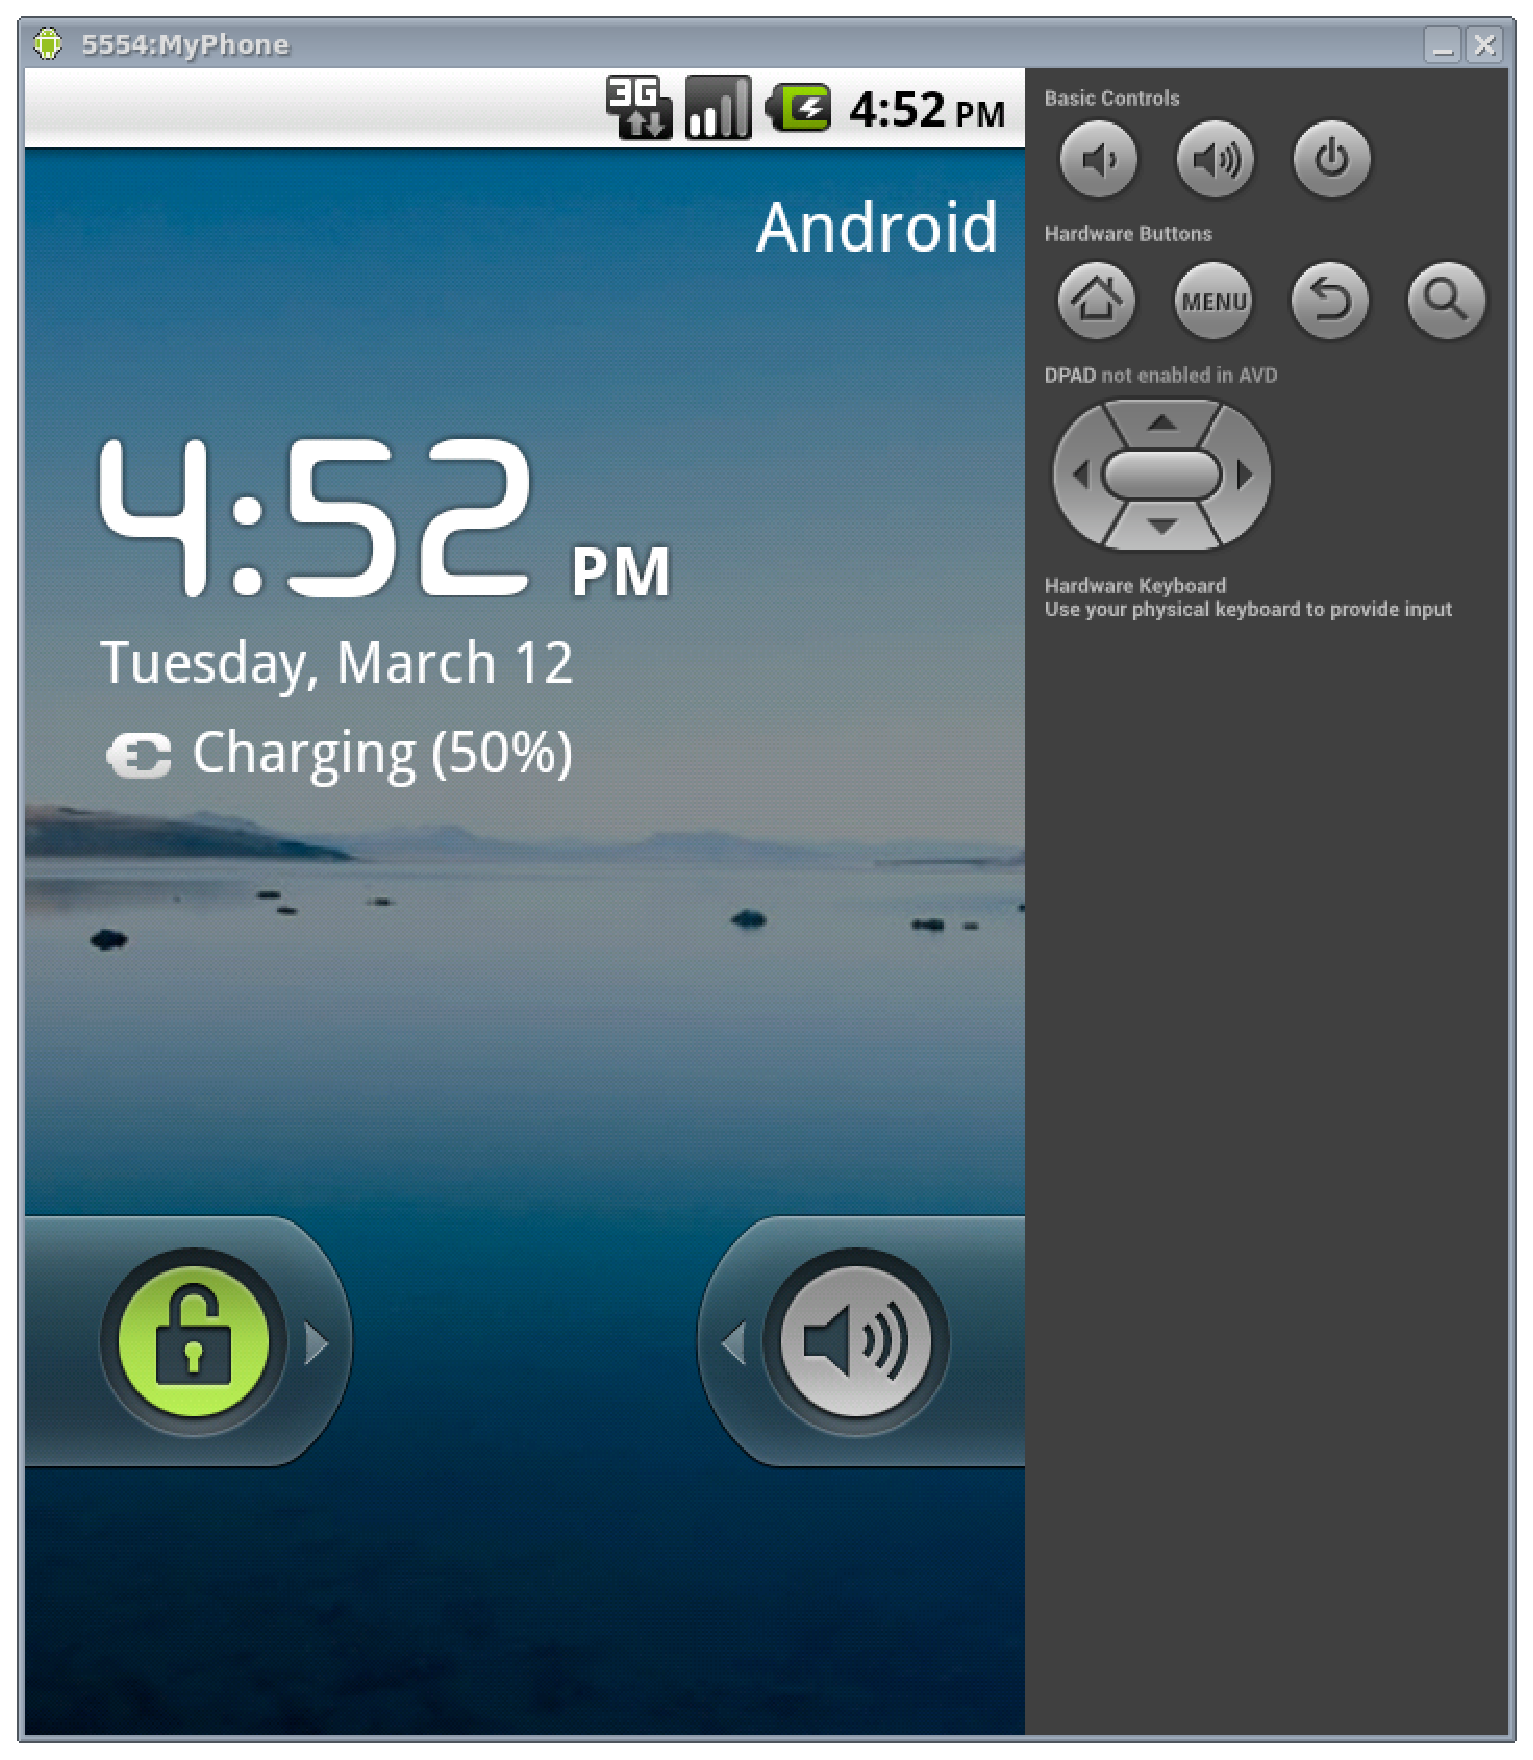
\includegraphics[width= 1.0 \textwidth]{MyPhone.eps}
\column{0.5 \textwidth}
\centering
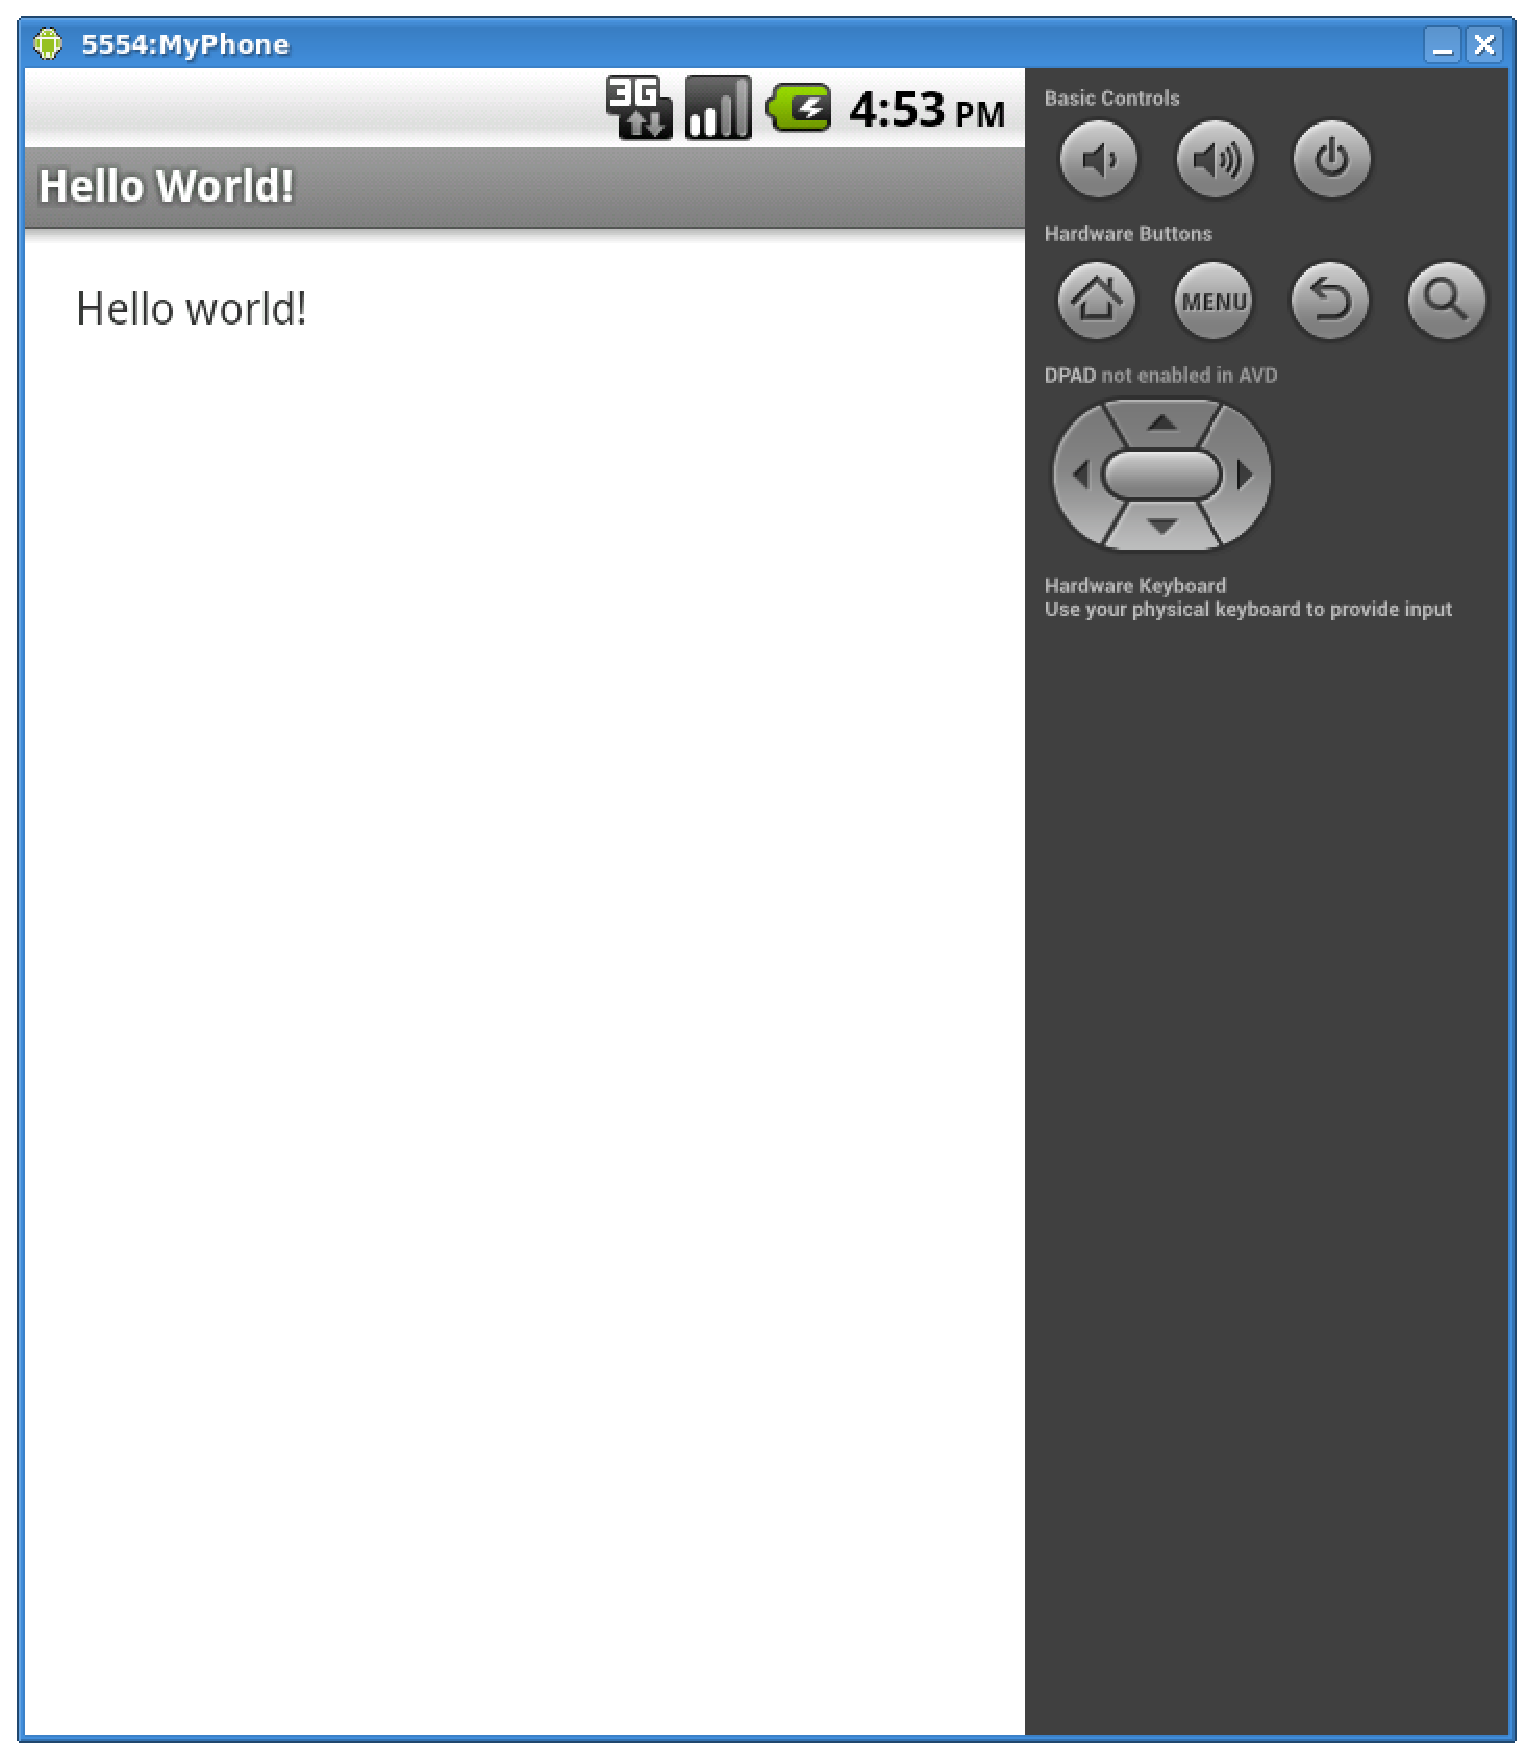
\includegraphics[width= 1.0 \textwidth]{HelloWorld.eps}
\end{columns}
\end{frame}
%------------------------------------------------------------------------------
\subsection{The Yamba Application}
%------------------------------------------------------------------------------
\begin{frame}
\frametitle{Yet Another Micro Blogging App}
\begin{columns}
 \column{0.33 \textwidth}
	\begin{figure}
	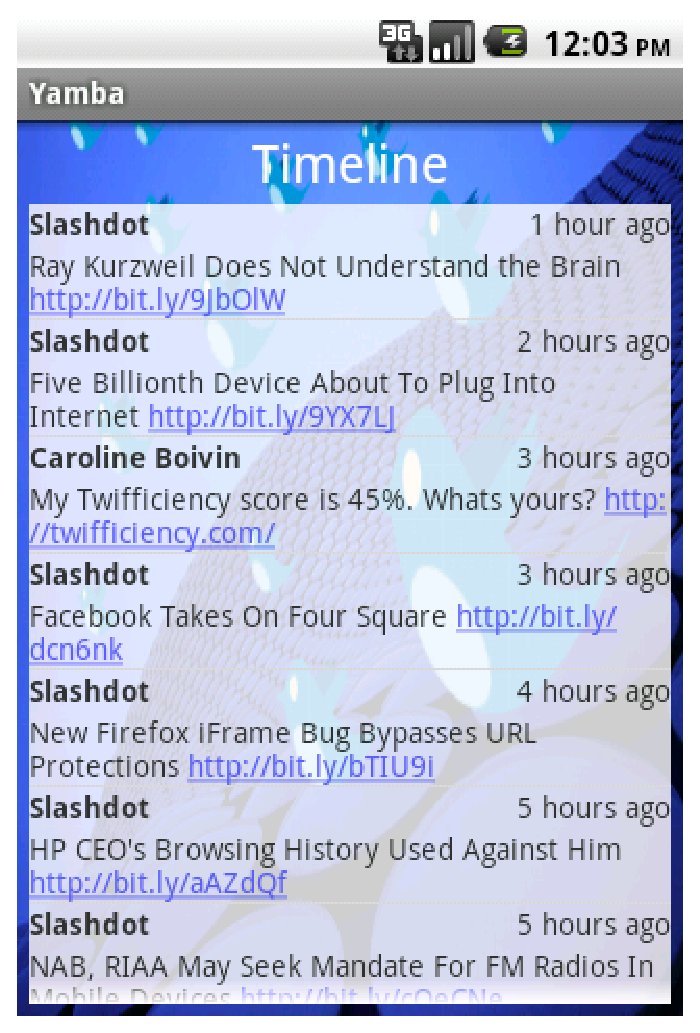
\includegraphics[width= 0.8 \textwidth]{fig-30.eps}
	\caption{List of status messages from other people, called a timeline}
	\end{figure}
 \column{0.33 \textwidth}
	\begin{figure}
	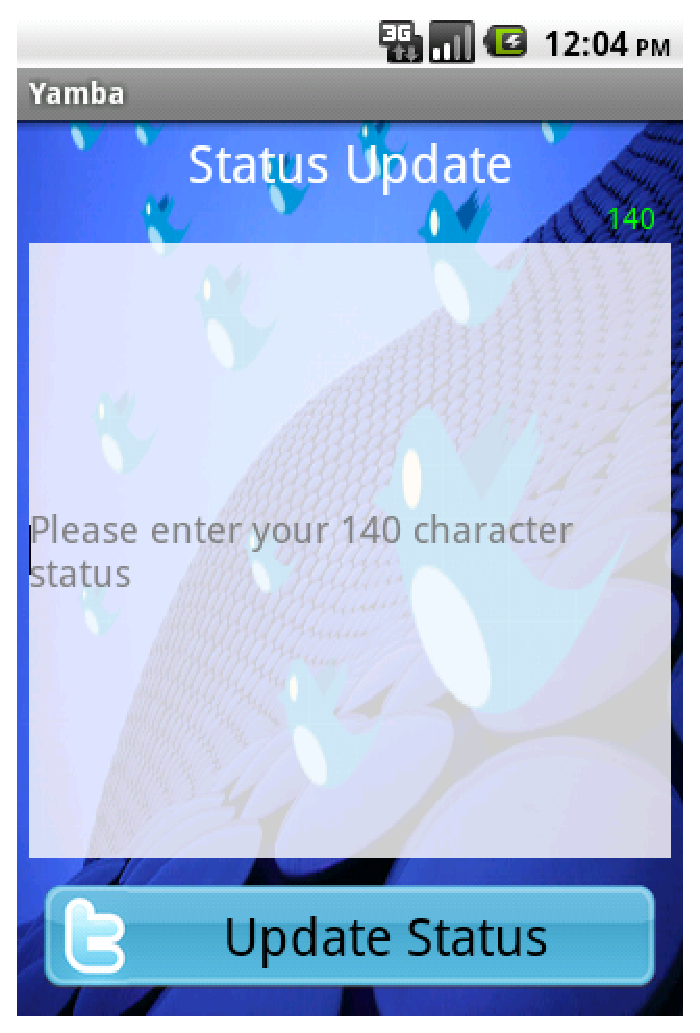
\includegraphics[width= 0.8 \textwidth]{fig-31.eps}
	\caption{Screen where the user can enter a status message}
	\end{figure}
 \column{0.34 \textwidth}
	\begin{figure}
	\includegraphics[width= 0.8 \textwidth]{fig-32.eps}
	\caption{User preferences}
	\end{figure}
\end{columns}

\end{frame}
%------------------------------------------------------------------------------

%%%%%%%%%%%%%%%%%%%%%%%%%%%%%%%%%%%%%%%%%%%%%%%%%%%%%%%%%%%%%%%%%%%%%%%%%%%%%%%%%
\section{Android User Interface}
%%%%%%%%%%%%%%%%%%%%%%%%%%%%%%%%%%%%%%%%%%%%%%%%%%%%%%%%%%%%%%%%%%%%%%%%%%%%%%%%
%------------------------------------------------------------------------------
\begin{frame}
\frametitle{Android User Interface}
\begin{columns}
 \column{0.33 \textwidth}
	\begin{figure}
	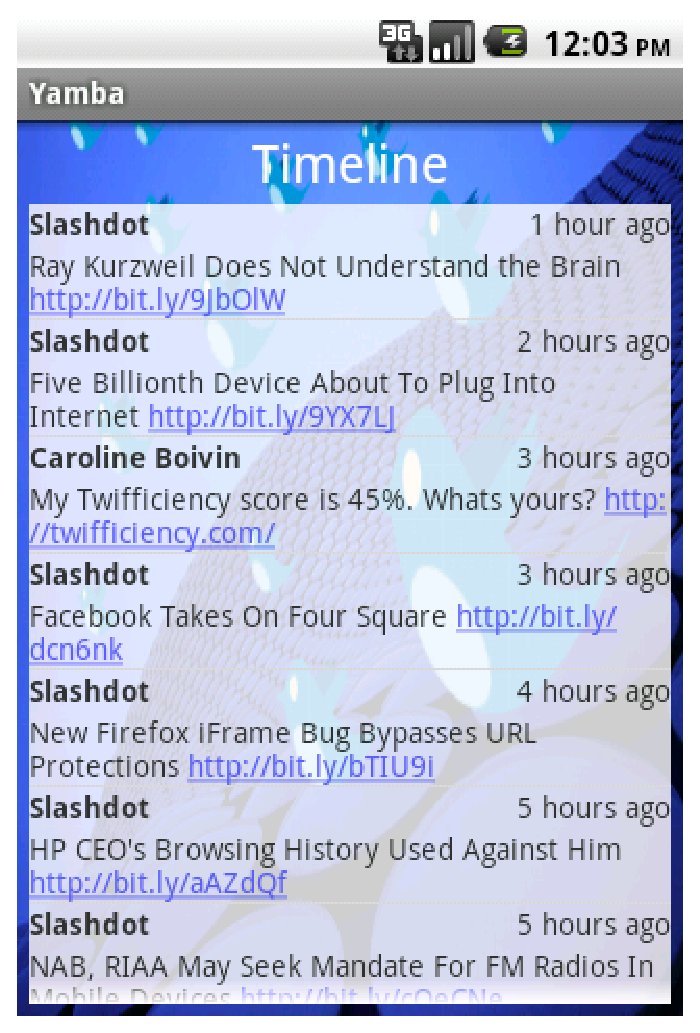
\includegraphics[width= 0.8 \textwidth]{fig-30.eps}
	\caption{List of status messages from other people, called a timeline}
	\end{figure}
 \column{0.33 \textwidth}
	\begin{figure}
	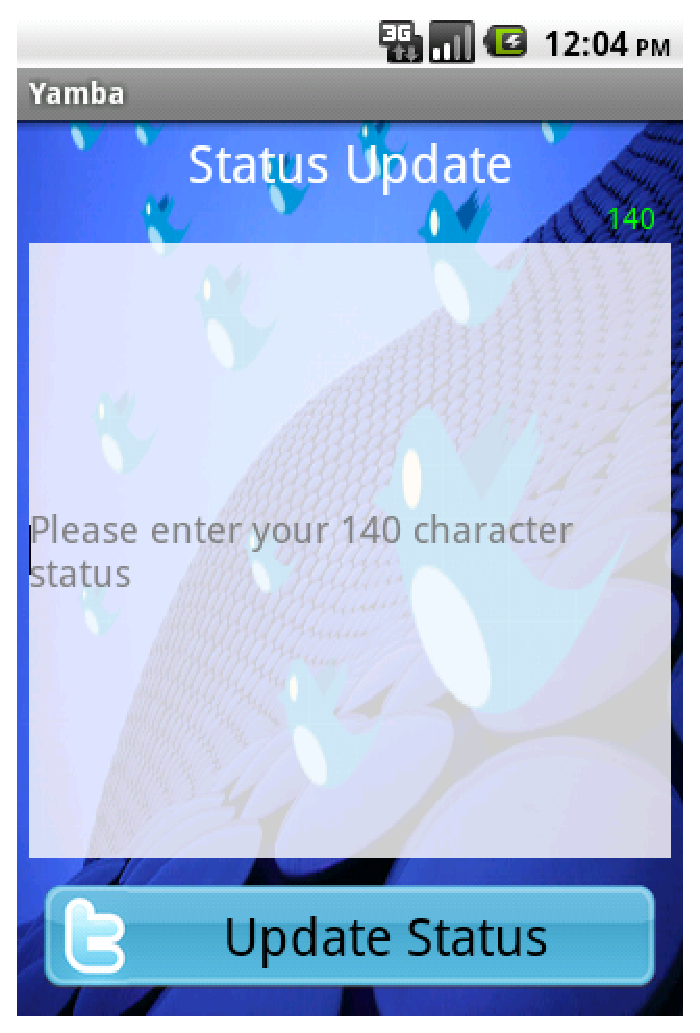
\includegraphics[width= 0.8 \textwidth]{fig-31.eps}
	\caption{Screen where the user can enter a status message}
	\end{figure}
 \column{0.34 \textwidth}
	\begin{figure}
	\includegraphics[width= 0.8 \textwidth]{fig-32.eps}
	\caption{User preferences}
	\end{figure}
\end{columns}

\end{frame}

%------------------------------------------------------------------------------
\subsection{Starting the Yamba Project}
\begin{frame}
\frametitle{Starting the Yamba Project}
File|New Android Application Project\\
\begin{columns}
\column{0.5 \textwidth}
	\begin{figure}
	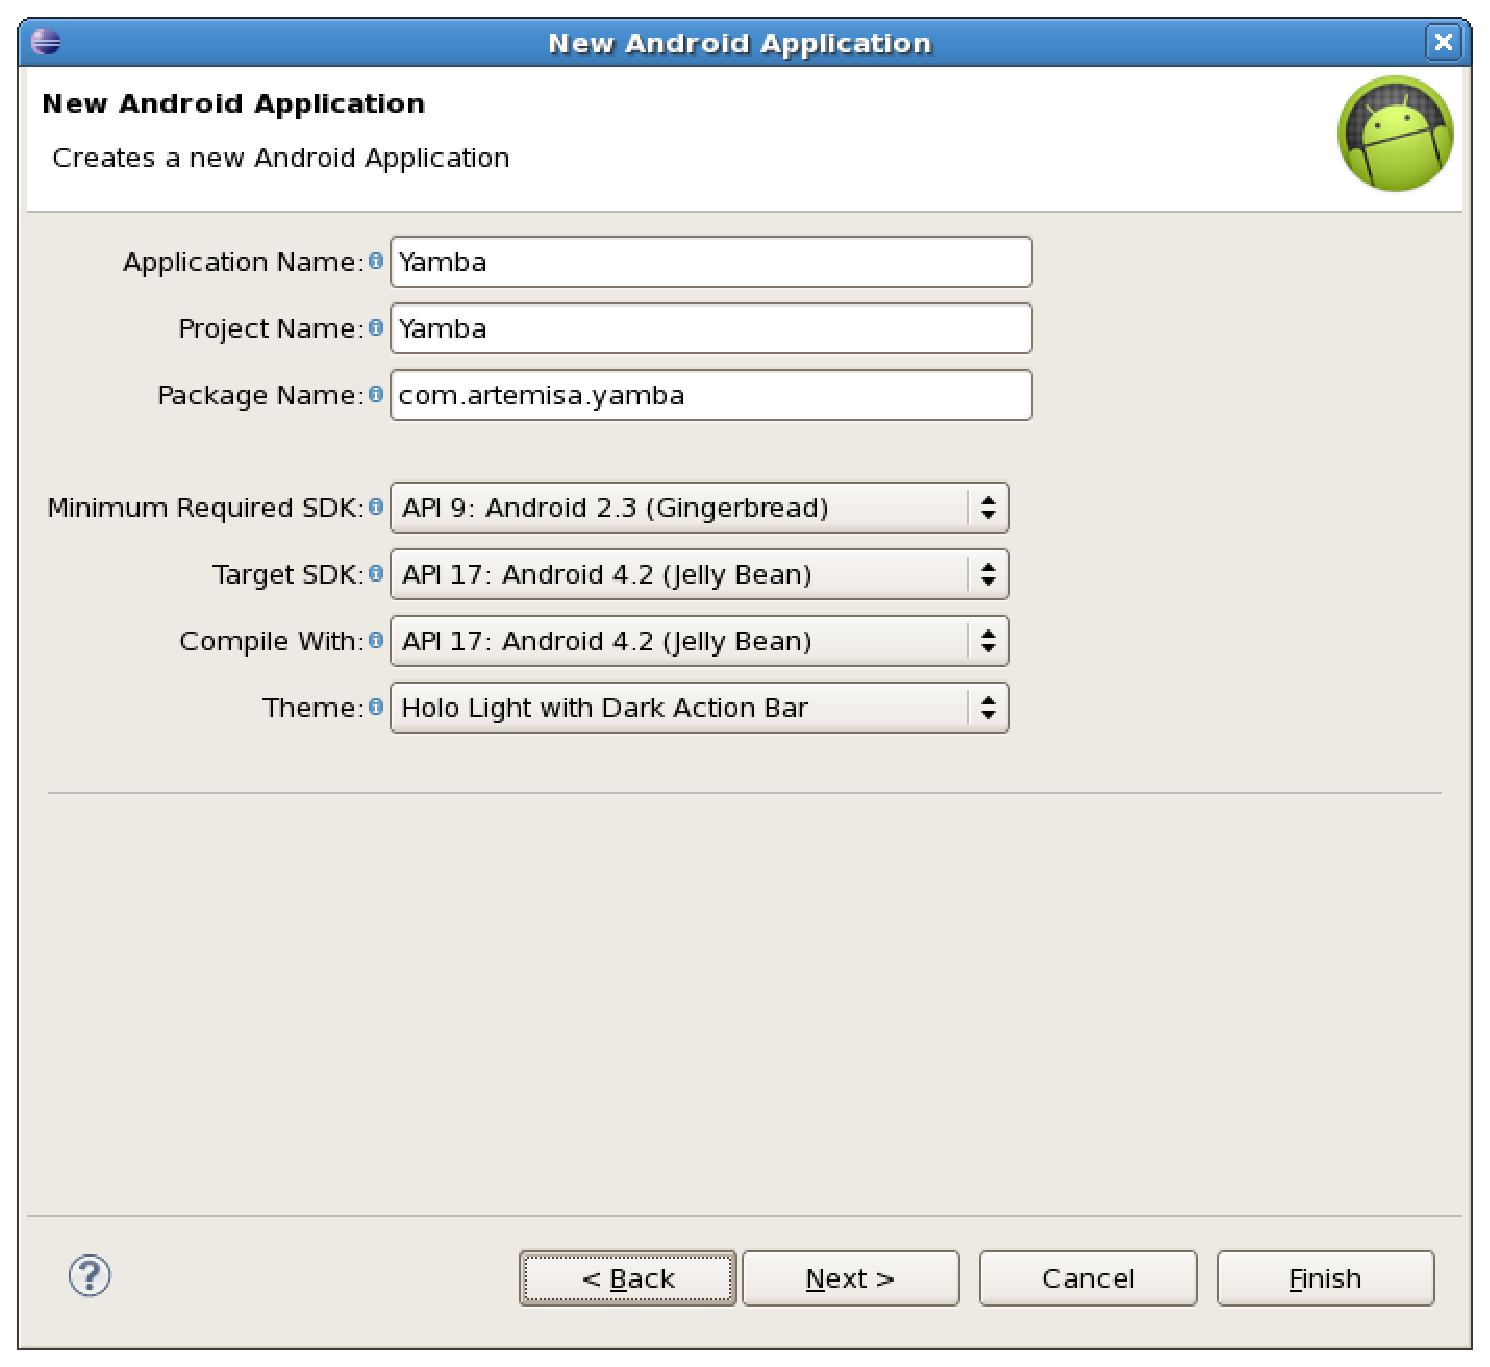
\includegraphics[width= 0.8 \textwidth]{yambaNewAndroidApplication1.eps}
	\caption{Application Name \texttt{Yamba}, Project Name \texttt{Yamba} and Package Name \texttt{com/artemisa/yamba}}
	\end{figure}
 \column{0.5 \textwidth}
	\begin{figure}
	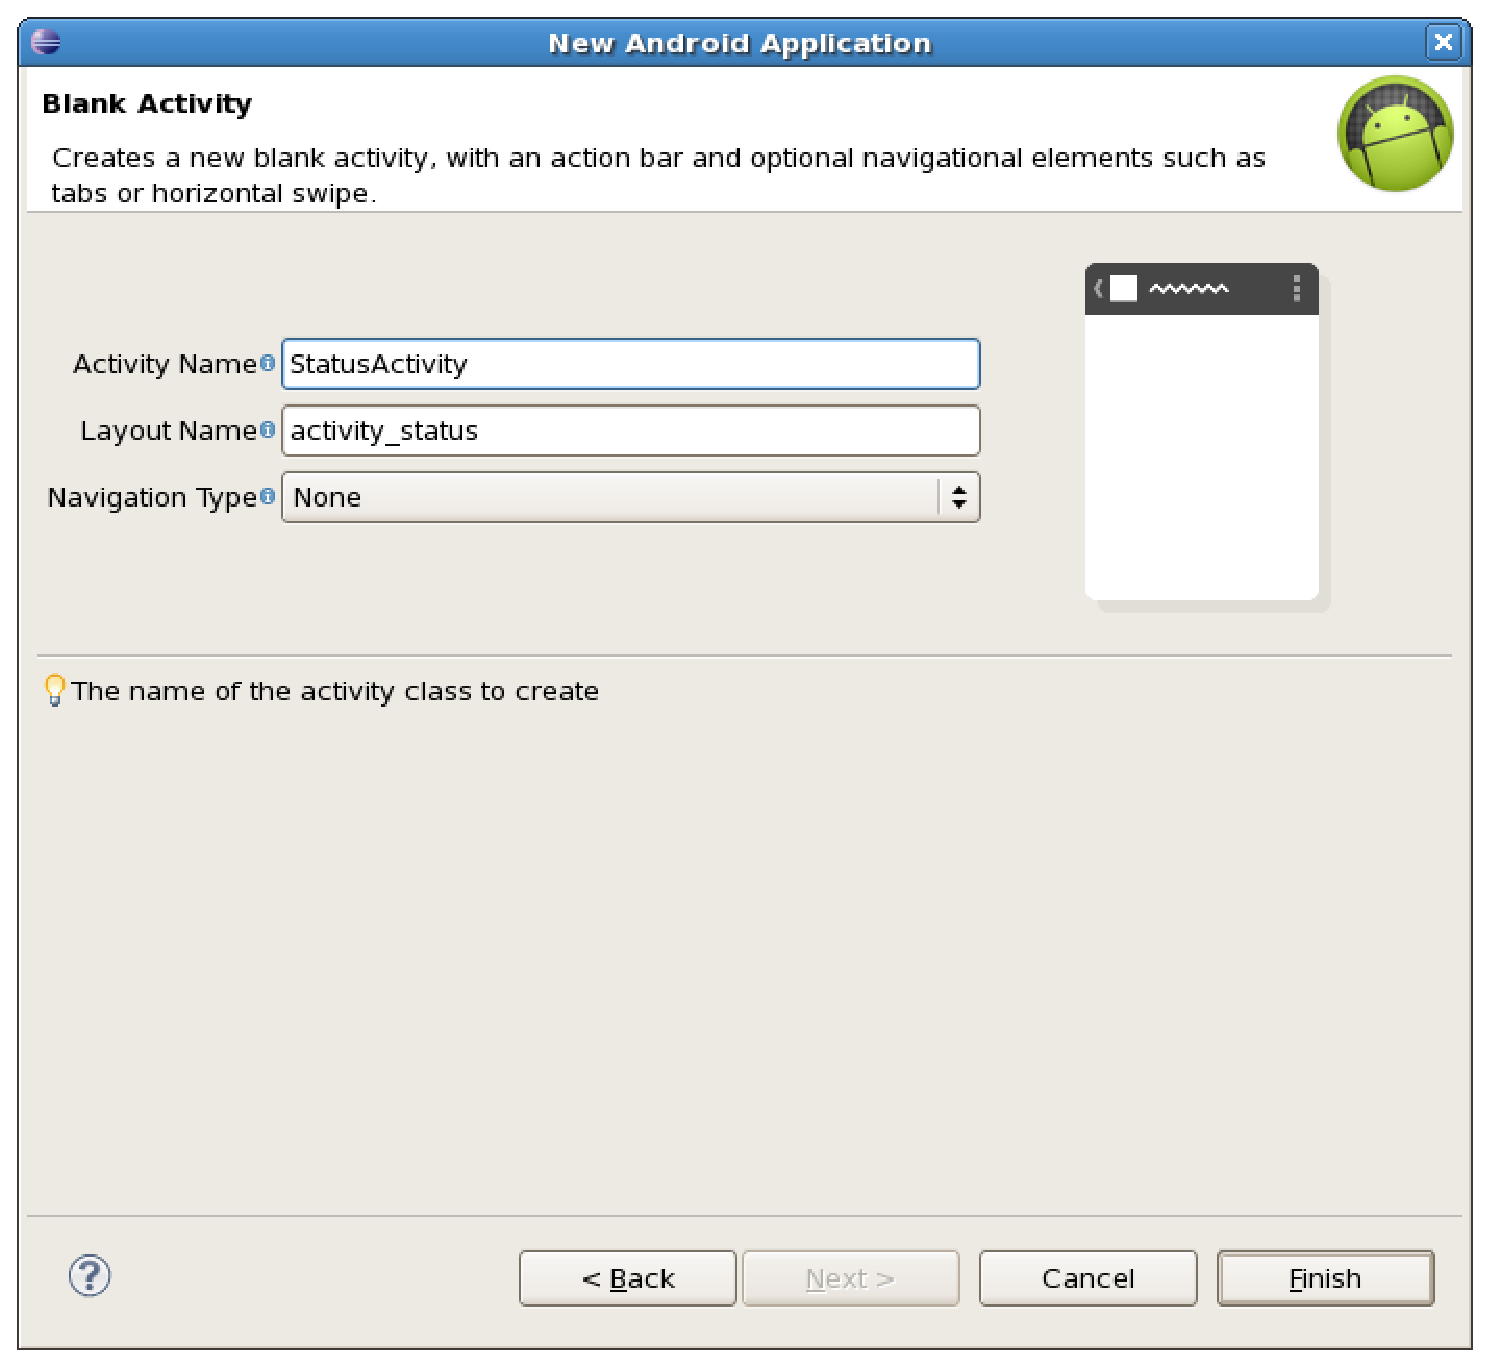
\includegraphics[width= 0.8 \textwidth]{yambaNewAndroidApplication2.eps}
	\caption{Activity Name \texttt{StatusActivity} and Layout Name \texttt{activity\_status}}
	\end{figure}
\end{columns}
\end{frame}
%------------------------------------------------------------------------------
\subsection{Git}
\begin{frame}
\frametitle{Git}
\begin{enumerate}
\item Fisrt Time System Setup
	\begin{enumerate}
 		\item \texttt{git config --global user.name "Juan García"}
 		\item \texttt{git config --global user.email juangarcia@mailinator.com}
	\end{enumerate}
\item First Time Repository Setup
	\begin{enumerate}
		\item Define \texttt{.gitignore}
		\item \texttt{git init}
	\end{enumerate}
\item Adding and Committing
	\begin{enumerate}
		\item \texttt{git add .}
		\item \texttt{git status}
		\item \texttt{git commit -m  ``Initial commit''}
	\end{enumerate}

\end{enumerate}
\end{frame}
%------------------------------------------------------------------------------
\subsection{The StatusActivity Layout}
\begin{frame}
\frametitle{The StatusActivity Layout}
\begin{columns}
 \column{0.65 \textwidth}
This screen will have four components
\begin{enumerate}
	\item A title at the top of the screen. \texttt{TextView} widget
	\item A big text area to type our 140-character status update. \texttt{EditText} widget
	\item A button to click to update the status. \texttt{Button} widget
	\item A layout to contain all these widgets and lay them out one after another in a vertical fashion. \texttt{LinearLayout}
\end{enumerate}
\column{0.35 \textwidth}
	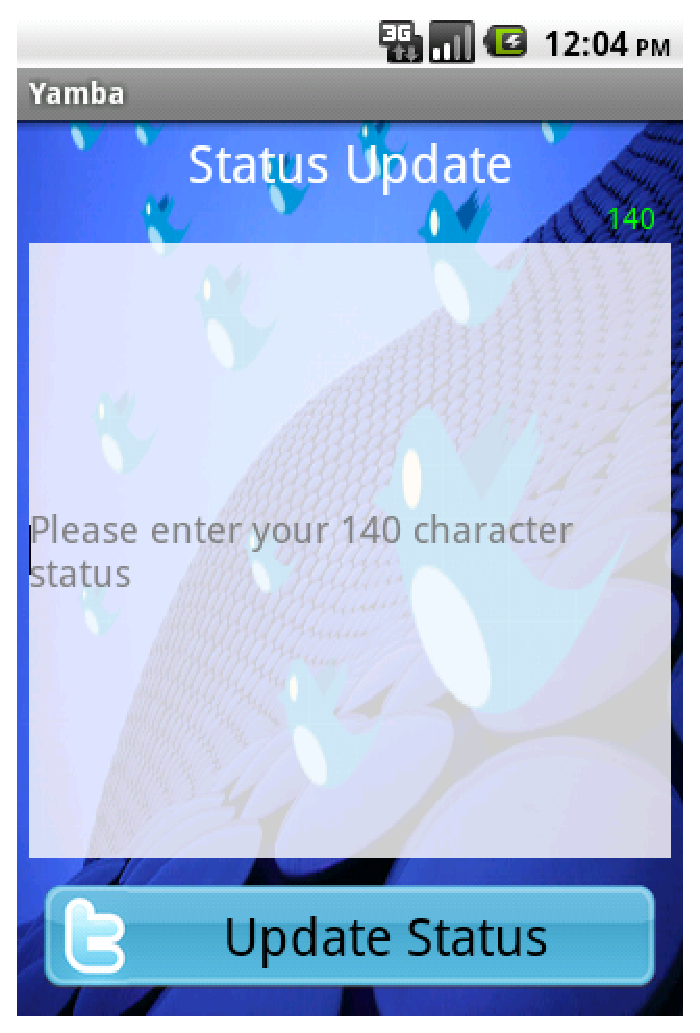
\includegraphics[width= 0.8 \textwidth]{fig-31.eps}
\end{columns}

\end{frame}
%------------------------------------------------------------------------------
\begin{frame}[allowframebreaks,containsverbatim]
\frametitle{Layout XML Code}
This code was generated by Eclipse Graphical Layout
\lstset{language=XML, style=eclipse}
%\begin{adjustbox}{width=1.0 \textwidth}
\begin{lstlisting}[caption=res/layout/activity\_status.xml, basicstyle=\scriptsize,escapechar=!]
<LinearLayout xmlns:android="http://schemas.android.com/apk/res/android"
    xmlns:tools="http://schemas.android.com/tools"
    android:id="@+id/LinearLayout"
    !\colorbox{light-gray}{android:layout\_width="fill\_parent"}!
    !\colorbox{light-gray}{android:layout\_height="fill\_parent"}!
    !\colorbox{light-gray}{android:orientation="vertical"}!
    android:paddingBottom="@dimen/activity_vertical_margin"
    android:paddingLeft="@dimen/activity_horizontal_margin"
    android:paddingRight="@dimen/activity_horizontal_margin"
    android:paddingTop="@dimen/activity_vertical_margin"
    tools:context=".StatusActivity" > !\pagebreak!

    <TextView
        !\colorbox{light-gray}{android:layout\_width="fill\_parent"}!
        !\colorbox{light-gray}{android:layout\_height="wrap\_content"}!
        !\colorbox{light-gray}{android:layout\_margin="10dp"}!
        !\colorbox{light-gray}{android:gravity="center"}!
        !\colorbox{light-gray}{android:text="@string/titleStatus"}!
        !\colorbox{light-gray}{android:textSize="30sp"}! /> !\pagebreak!

    <EditText
        android:id="@+id/editText"
        !\colorbox{light-gray}{android:layout\_width="fill\_parent"}!
        !\colorbox{light-gray}{android:layout\_height="fill\_parent"}!
        !\colorbox{light-gray}{android:layout\_weight="1"}!
        android:ems="10"
        !\colorbox{light-gray}{android:gravity="top|left"}!
        !\colorbox{light-gray}{android:hint="@string/hintText"}! >
        <requestFocus />
    </EditText> !\pagebreak!

    <Button
        !\colorbox{light-gray}{android:id="@+id/buttonUpdate"}!
        !\colorbox{light-gray}{android:layout\_width="fill\_parent"}!
        !\colorbox{light-gray}{android:layout\_height="wrap\_content"}!
        !\colorbox{light-gray}{android:text="@string/buttonUpdate"}!
        !\colorbox{light-gray}{android:textSize="20sp"}! />

</LinearLayout>
\end{lstlisting}
%\end{adjustbox}
\end{frame}
%------------------------------------------------------------------------------
\begin{frame}
\frametitle{Important Widget Properties}
\begin{description}
	\item[\texttt{layout\_height} and \texttt{layout\_width}] Defines how much space this widget is asking from its parent layout to display
itself. Best practice would be to use either \texttt{fill\_parent} or \texttt{wrap\_content} for the value
	\item[\texttt{layout\_gravity}]Specifies how this particular widget is positioned within its layout, both horizontally
and vertically. \texttt{top}, \texttt{center}, \texttt{left} \dots
	\item[\texttt{gravity}] Specifies how the content of this widget is positioned within the widget itself
	\item[\texttt{text}] It simply specifies the text for the widget
	\item[\texttt{id}] \texttt{id} is simply the unique identifier for this particular widget in a particular layout resource file
\end{description}
\end{frame}
%------------------------------------------------------------------------------
\begin{frame}[fragile]
\frametitle{Strings Resource}
\lstset{language=XML, style=eclipse}
\begin{adjustbox}{width=1.0 \textwidth}
\centering
\begin{lstlisting}[caption=res/values/strings.xml]
<?xml version="1.0" encoding="utf-8"?>
<resources>
    <string name="app_name">Yamba</string>
    <string name="action_settings">Settings</string>
    <string name="hello_world">Hello world!</string>
    <string name="titleStatus">Status Update</string>

    <string name="hintText">Please entrer your 140-character status</string>

    <string name="buttonUpdate">Update</string>
</resources>
\end{lstlisting}
\end{adjustbox}
\end{frame}


%------------------------------------------------------------------------------
\begin{frame}[fragile]
\frametitle{Observer Pattern}
\url{http://en.wikipedia.org/wiki/Observer_pattern}\\
\begin{columns}
\column{1.0 \textwidth}
	\begin{figure}
	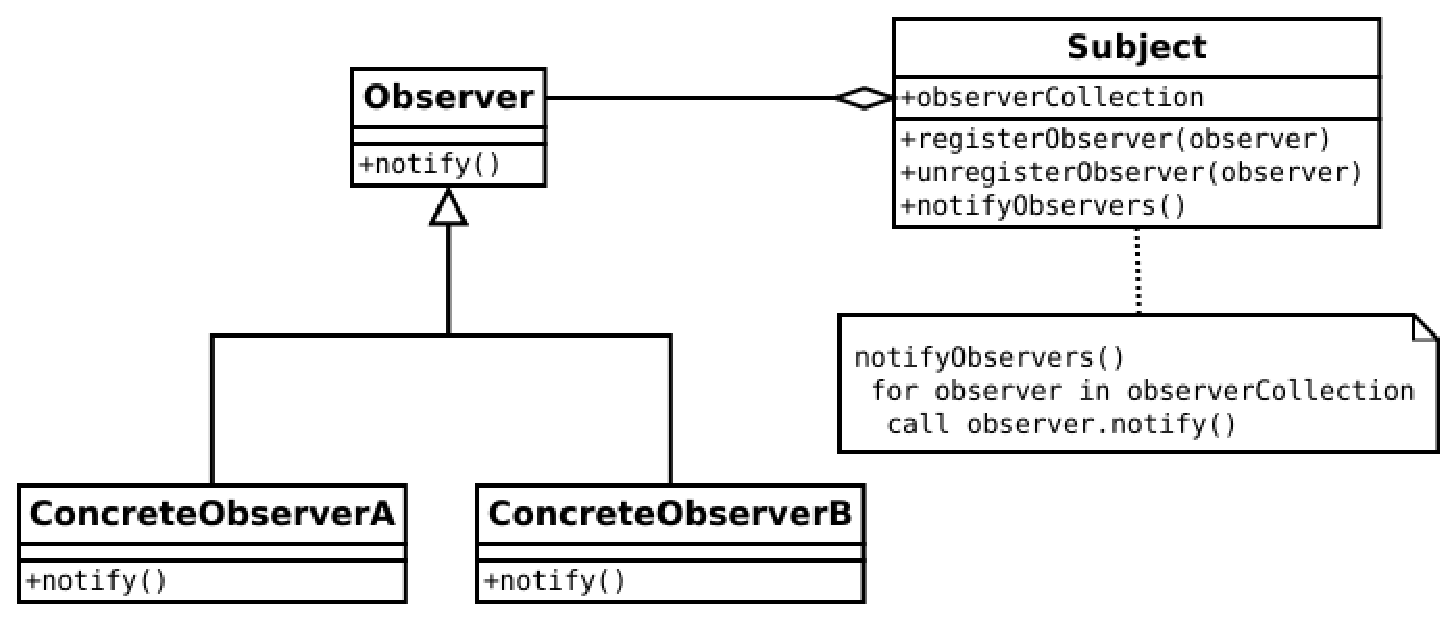
\includegraphics[width= 1.0 \textwidth]{observer.eps}
	\caption{UML class diagram of Observer pattern}
	\end{figure}
\end{columns}
\end{frame}
%------------------------------------------------------------------------------
\begin{frame}[allowframebreaks,containsverbatim]
\frametitle{The StatusActivity Java Class}
\lstset{language=java, style=eclipse, breaklines=true, tabsize=2}
%\begin{adjustbox}{width=1.0 \textwidth}
\centering
\begin{lstlisting}[caption=src/com/artemisa/yamba/StatusActivity.java, basicstyle=\tiny, escapechar=! ]
// .
// .
// .
public class StatusActivity extends Activity implements OnClickListener { // !\circled{1}!

	private static final String TAG = "Status Activity";
	private Button updateButton;
	private EditText editText;

	@Override
	protected void onCreate(Bundle savedInstanceState) {
		super.onCreate(savedInstanceState);
		setContentView(R.layout.activity_status);

		// Find views and set Observer !\circled{2}!
		updateButton = (Button) findViewById(R.id.buttonUpdate);
		updateButton.setOnClickListener(this);

		editText = (EditText) findViewById(R.id.editText);
	}

	@Override
	public boolean onCreateOptionsMenu(Menu menu) {
		// Inflate the menu; this adds items to the action bar if it is present.
		getMenuInflater().inflate(R.menu.status, menu);
		return true;
	}

	// Called whe button is clicked !\circled{3}!
	public void onClick(View v) {
		Log.d(TAG, "OnClic:" + editText.getText().toString());
	}

}

\end{lstlisting}
%\end{adjustbox}
\end{frame}
%------------------------------------------------------------------------------
\begin{frame}[fragile]
\frametitle{Git}
\begin{enumerate}
\item \texttt{git status}
\item \texttt{git commit -a -m ``OnClickListener''}

\end{enumerate}


\end{frame}
%------------------------------------------------------------------------------
\subsection{Connecting on Twitter}

\begin{frame}[fragile]
\frametitle{Connecting on Twitter}
\url{http://yamba.maracana.com}

To make our life with web services and the Twitter API easier, we’re going to use a
third-party library, \href{http://www.winterwell.com/software/jtwitter.php}{jtwitter.jar}, provided by Winterwell Associates

\begin{itemize}
 \item Once you download this library, you can put it inside your project in Eclipse. Copy \texttt{jtwitter-yamba.jar} in \texttt{libs} directory
 \item Add \texttt{jtwitter-yamba.jar} to the \alert{classpath}, right-click on your project, select Properties, and you will get a Properties for Yamba
dialog window. Select Java Build Path, and choose the Libraries tab. In there, click on Add External JARs… and locate your jtwitter.jar file

\end{itemize}

\end{frame}
%------------------------------------------------------------------------------
\begin{frame}[fragile]
\frametitle{Updating the Manifest File for Internet Permission}
\lstset{language=XML, style=eclipse}
\begin{adjustbox}{width=0.75 \textwidth}
\centering
\begin{lstlisting}[caption=AndroidManifest.xml,basicstyle=\tiny, escapechar=$]
<?xml version="1.0" encoding="utf-8"?>
<manifest xmlns:android="http://schemas.android.com/apk/res/android"
    package="com/artemisa/yamba1"
    android:versionCode="1"
    android:versionName="1.0" >

    <uses-sdk
        android:minSdkVersion="8"
        android:targetSdkVersion="17" />
    <uses-permission android:name="android.permission.INTERNET" /> <!-- $\circled{1}$ -->
	
    <application
        android:allowBackup="true"
        android:icon="@drawable/ic_launcher"
        android:label="@string/app_name"
        android:theme="@style/AppTheme" >
        <activity
            android:name="com/artemisa/yamba1.StatusActivity"
            android:label="@string/app_name" >
            <intent-filter>
                <action android:name="android.intent.action.MAIN" />

                <category android:name="android.intent.category.LAUNCHER" />
            </intent-filter>
        </activity>
    </application>

</manifest>
\end{lstlisting}
\end{adjustbox}
\end{frame}
%------------------------------------------------------------------------------

\begin{frame}[allowframebreaks,containsverbatim]
\frametitle{The StatusActivity Java Class}
\lstset{language=java, style=eclipse, breaklines=true, tabsize=2}
%\begin{adjustbox}{width=1.0 \textwidth}
\centering
\begin{lstlisting}[caption=src/com/artemisa/yamba/StatusActivity.java, basicstyle=\tiny, escapechar=!, ]
// .
// .
// .
public class StatusActivity extends Activity implements OnClickListener {
	private static final String TAG = "StatusActivity";
	private Button updateButton;
	private EditText editText;
	private Twitter twitter; // !\circled{1}!

	@Override
	protected void onCreate(Bundle savedInstanceState) {
		super.onCreate(savedInstanceState);
		setContentView(R.layout.activity_status);
	
		// Find views
		updateButton = (Button) findViewById(R.id.buttonUpdate);
		updateButton.setOnClickListener(this);
	
		editText = (EditText) findViewById(R.id.editText);
	
		twitter = new Twitter("student", "password"); // !\circled{2}!
		twitter.setAPIRootUrl("http://yamba.marakana.com/api");
	}

	@Override
	public boolean onCreateOptionsMenu(Menu menu) {
		// Inflate the menu; this adds items to the action bar if it is present.
		getMenuInflater().inflate(R.menu.status, menu);
		return true;
	}

	// Called when button is clicked
	public void onClick(View v) { // !\circled{4}!
		try {
			twitter.setStatus(editText.getText().toString());
			Log.d(TAG, "OnCLick: " + editText.getText().toString());
		} catch (TwitterException e) {
			Log.e(TAG, e.toString());
			e.printStackTrace();
		}
	}

}

\end{lstlisting}
%\end{adjustbox}
\end{frame}

%------------------------------------------------------------------------------

\begin{frame}[fragile]
\frametitle{Git}
\begin{enumerate}
\item \texttt{git status}
\item \texttt{git commit -a -m ``Connecting on Twitter''}

\end{enumerate}

\end{frame}
%------------------------------------------------------------------------------
\subsection{Toast}

\begin{frame}[fragile]
\frametitle{Toast}

\lstset{language=java, style=eclipse, breaklines=true, tabsize=2}
A toast provides simple feedback about an operation in a small popup. It only fills the amount of space required for the message and the current activity remains visible and interactive. 
\begin{lstlisting}
Context context = getApplicationContext();
CharSequence text = "Hello toast!";
int duration = Toast.LENGTH_SHORT;

Toast toast = Toast.makeText(context, text, duration);
toast.show();
\end{lstlisting}
\end{frame}
%------------------------------------------------------------------------------



\subsection{Asynchronous Threads}
\begin{frame}[fragile]
\frametitle{Asynchronous Task }

\lstset{language=java, style=eclipse, breaklines=true, tabsize=2}
\centering
\lstinline{private class MyTask extends AsyncTask<Params, Progress, Result> }

\begin{itemize}
\item An asynchronous task is defined by 3 generic types: \lstinline{Params}, \lstinline{Progress}, \lstinline{Result}

\item And 4 steps:
\lstinline{void onPreExecute()}, \lstinline{Result doInBackground(Params...)}, \lstinline{void onProgressUpdate(Progress...)}, \lstinline{void onPostExecute(Result)}

\item The task instance must be created on the UI thread. \lstinline{execute(Params...)} must be invoked on the UI thread

\item We need to create a new inner subclass \lstinline{PostToTwitter} of \lstinline{AsyncTask} and implement all methods. The \lstinline{PostToTwitter} class in this case will be an inner class of \lstinline{StatusActivity}

\end{itemize}

\end{frame}

%------------------------------------------------------------------------------



\begin{frame}[allowframebreaks,containsverbatim]
\frametitle{The StatusActivity Java Class}
\lstset{language=java, style=eclipse, breaklines=true, tabsize=2}
\begin{lstlisting}[caption=src/com/artemisa/yamba/StatusActivity.java, basicstyle=\tiny, escapechar=! ]
// .
// .
// .
public class StatusActivity extends Activity implements OnClickListener {
	// .
	// .
	// .
	// Asynchronously posts to twitter
	class PostToTwitter extends AsyncTask<String, Integer, String> { !\circled{1}!
		// Called to initiate the background activity
		@Override
		protected String doInBackground(String... statuses) { !\circled{2}!
			try {
				Twitter.Status status = twitter.updateStatus(statuses[0]);
				return status.text;
			} catch (TwitterException e) {
				Log.e(TAG, e.toString());
				e.printStackTrace();
				return "Failed to post";
			}
		} !\linebreak!

		// Called when there's a status to be updated
		@Override
		protected void onProgressUpdate(Integer... values) { !\circled{3}!
			super.onProgressUpdate(values);
			// Not used in this case
		}

		// Called when the background activity has completed
		@Override
		protected void onPostExecute(String result) { !\circled{4}!
			Toast.makeText(getApplicationContext(), result, Toast.LENGTH_SHORT)
					.show();
		} !\linebreak!
	}

	// Called when button is clicked
	public void onClick(View v) { !\circled{5}!
		String status = editText.getText().toString();
		new PostToTwitter().execute(status);
	} 

}
\end{lstlisting}
\end{frame}
%------------------------------------------------------------------------------
\begin{frame}[fragile]
\frametitle{Git}
\begin{enumerate}
\item \texttt{git status}
\item \texttt{git commit -a -m ``Asynchronous Threads''}
\end{enumerate}

\end{frame}
%------------------------------------------------------------------------------






\subsection{Other UI Events}
%------------------------------------------------------------------------------
\begin{frame}[fragile]
\centering
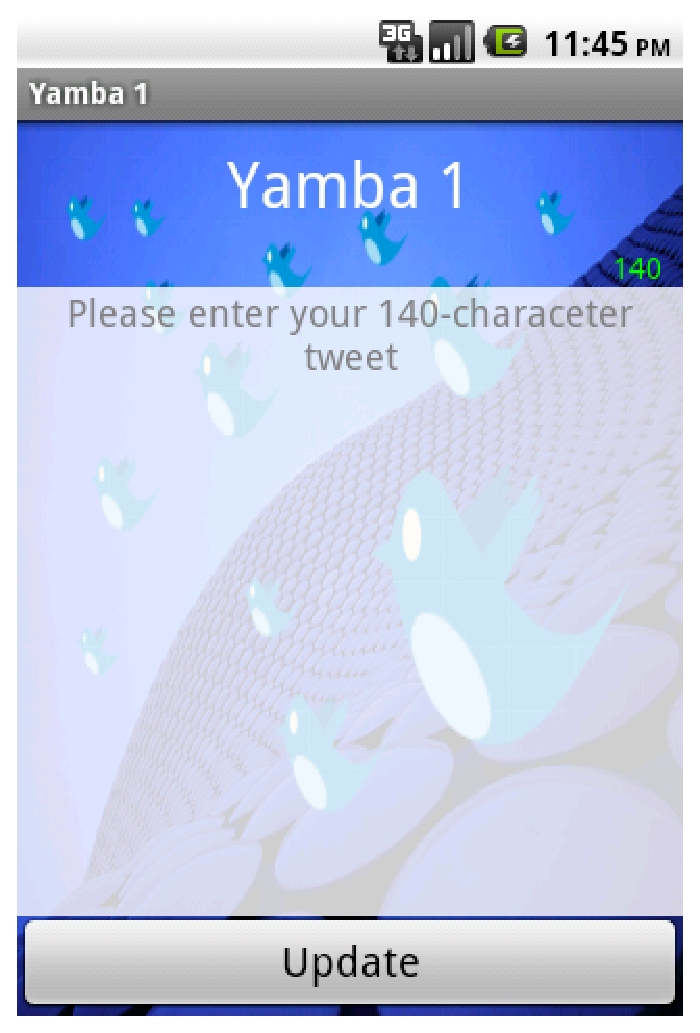
\includegraphics[width=0.4 \textwidth]{fig-063.eps}

\end{frame}
%------------------------------------------------------------------------------
\begin{frame}[allowframebreaks,containsverbatim]
\frametitle{activity\_status.xml}
\begin{itemize}
\item We’ll add another \texttt{TextView} to our layout to indicate how
many characters are still available. This text will change color, from green to yellow to
red
\lstset{language=XML, style=eclipse}
\begin{adjustbox}{width=0.8 \textwidth}
\begin{lstlisting}[caption=activity\_status.xml, escapechar=!]
<TextView
        android:id="@+id/textCount"
        android:layout_width="wrap_content"
        android:layout_height="wrap_content"
        android:layout_gravity="right"
        android:layout_marginRight="10dp"
        android:text="000" />
\end{lstlisting}
\end{adjustbox}
\end{itemize}

\end{frame}
%------------------------------------------------------------------------------
\begin{frame}[containsverbatim]
\frametitle{TextWatcher Interface}
\begin{itemize}
\item \texttt{TextWatcher} interface to watch for text changes

\end{itemize}

\lstset{language=java, style=eclipse, breaklines=true, tabsize=2, basicstyle=\footnotesize , numbers=none}
\begin{lstlisting}
void afterTextChanged(Editable s)
void beforeTextChanged(CharSequence s, int start, int count, int after)
void onTextChanged(CharSequence s, int start, int before, int count)
\end{lstlisting}
\end{frame}
%------------------------------------------------------------------------------
%------------------------------------------------------------------------------
\begin{frame}[allowframebreaks,containsverbatim]
\frametitle{The StatusActivity Java Class}
\lstset{language=java, style=eclipse, breaklines=true, tabsize=2}
\begin{lstlisting}[caption=src/com/artemisa/yamba/StatusActivity.java, basicstyle=\tiny, escapechar=! ]
// .
// .
// .
public class StatusActivity extends Activity implements OnClickListener,
		TextWatcher { // !\circled{1}!
	private static final String TAG = "StatusActivity";
	private Button updateButton;
	private EditText editText; 
	private Twitter twitter;
	private TextView textCount; // !\circled{2}!

	@Override
	protected void onCreate(Bundle savedInstanceState) {
		super.onCreate(savedInstanceState);
		setContentView(R.layout.activity_status);

		// Find views
		updateButton = (Button) findViewById(R.id.buttonUpdate);
		updateButton.setOnClickListener(this);

		editText = (EditText) findViewById(R.id.editText);
		editText.addTextChangedListener(this); // !\circled{3}! 

		textCount = (TextView) findViewById(R.id.textCount); // !\circled{4}!
		textCount.setText(Integer.toString(140)); 
		textCount.setTextColor(Color.GREEN);

		twitter = new Twitter("student", "password");
		twitter.setAPIRootUrl("http://yamba.marakana.com/api");
	}

	@Override
	public boolean onCreateOptionsMenu(Menu menu) {
		// Inflate the menu; this adds items to the action bar if it is present.
		getMenuInflater().inflate(R.menu.status, menu);
		return true;
	}
	
	// Asynchronously posts to twitter
	// .
	// .
	// .
	
	// Called when button is clicked
	public void onClick(View v) {
		String status = editText.getText().toString();
		new PostToTwitter().execute(status);
	}

	// Called when editText's text changes
	@Override
	public void afterTextChanged(Editable s) { // !\circled{5}!
		Log.d(TAG, "afterTextChanged()");

		int count = 140 - s.length();
		String text = Integer.toString(count);

		textCount.setText(text);

		if (count > 10) {
			textCount.setTextColor(Color.GREEN);
		} else {
			if (count >= 1 && count <= 10) {
				textCount.setTextColor(Color.YELLOW);
			} else {
				textCount.setTextColor(Color.RED);
			}
		}
	}

	
	@Override
	public void beforeTextChanged(CharSequence s, int start, int count,
			int after) {
		// not used
	}

	@Override
	public void onTextChanged(CharSequence s, int start, int before, int count) {
		// no used
	}
}

\end{lstlisting}
\end{frame}
%------------------------------------------------------------------------------

\begin{frame}[fragile]
\frametitle{Git}
\begin{enumerate}
\item \texttt{git status}
\item \texttt{git commit -a -m ``Other UI Events''}
\end{enumerate}

\end{frame}

%------------------------------------------------------------------------------
\subsection{Color and Graphics}
\begin{frame}[allowframebreaks,containsverbatim]
\frametitle{Color and Graphics}
\begin{itemize}
\item Create another drawable folder called simply \texttt{/res/drawable}
\item Add \texttt{background.png}
\end{itemize}

\lstset{language=XML, style=eclipse}
\begin{lstlisting}[caption=res/layout/activity\_status.xml, basicstyle=\scriptsize,escapechar=$]
<LinearLayout xmlns:android="http://schemas.android.com/apk/res/android"
    xmlns:tools="http://schemas.android.com/tools"
    android:id="@+id/LinearLayout"
    android:layout_width="fill_parent"
    android:layout_height="fill_parent"
    android:background="@drawable/background" <!-- $\circled{1}$ -->
    android:orientation="vertical"
    android:paddingBottom="@dimen/activity_vertical_margin"
    android:paddingLeft="@dimen/activity_horizontal_margin"
    android:paddingRight="@dimen/activity_horizontal_margin"
    android:paddingTop="@dimen/activity_vertical_margin"
    tools:context=".StatusActivity" > $\pagebreak$

    <TextView
        android:layout_width="fill_parent"
        android:layout_height="wrap_content"
        android:layout_margin="10dp"
        android:background="@android:color/white" <!-- $\circled{2}$ -->
        android:gravity="center"
        android:text="@string/titleStatus"
        android:textSize="30sp" />

    <TextView
        android:id="@+id/textCount"
        android:layout_width="wrap_content"
        android:layout_height="wrap_content"
        android:layout_gravity="right"
        android:layout_marginRight="10dp"
        android:text="000" /> $\pagebreak$
	
    <EditText
        android:id="@+id/editText"
        android:layout_width="fill_parent"
        android:layout_height="fill_parent"
        android:layout_weight="1"
        android:background="#cfff" <!-- $\circled{3}$ -->
        android:ems="10"
        android:gravity="top|center_horizontal"
        android:hint="@string/hintText" >

        <requestFocus />
    </EditText> $\pagebreak$

    <Button
        android:id="@+id/buttonUpdate"
        android:layout_width="fill_parent"
        android:layout_height="wrap_content"
        android:text="@string/buttonUpdate"
        android:textSize="20sp" />

</LinearLayout>
\end{lstlisting}
\end{frame}
%------------------------------------------------------------------------------
\begin{frame}
\frametitle{Summary}
\centering
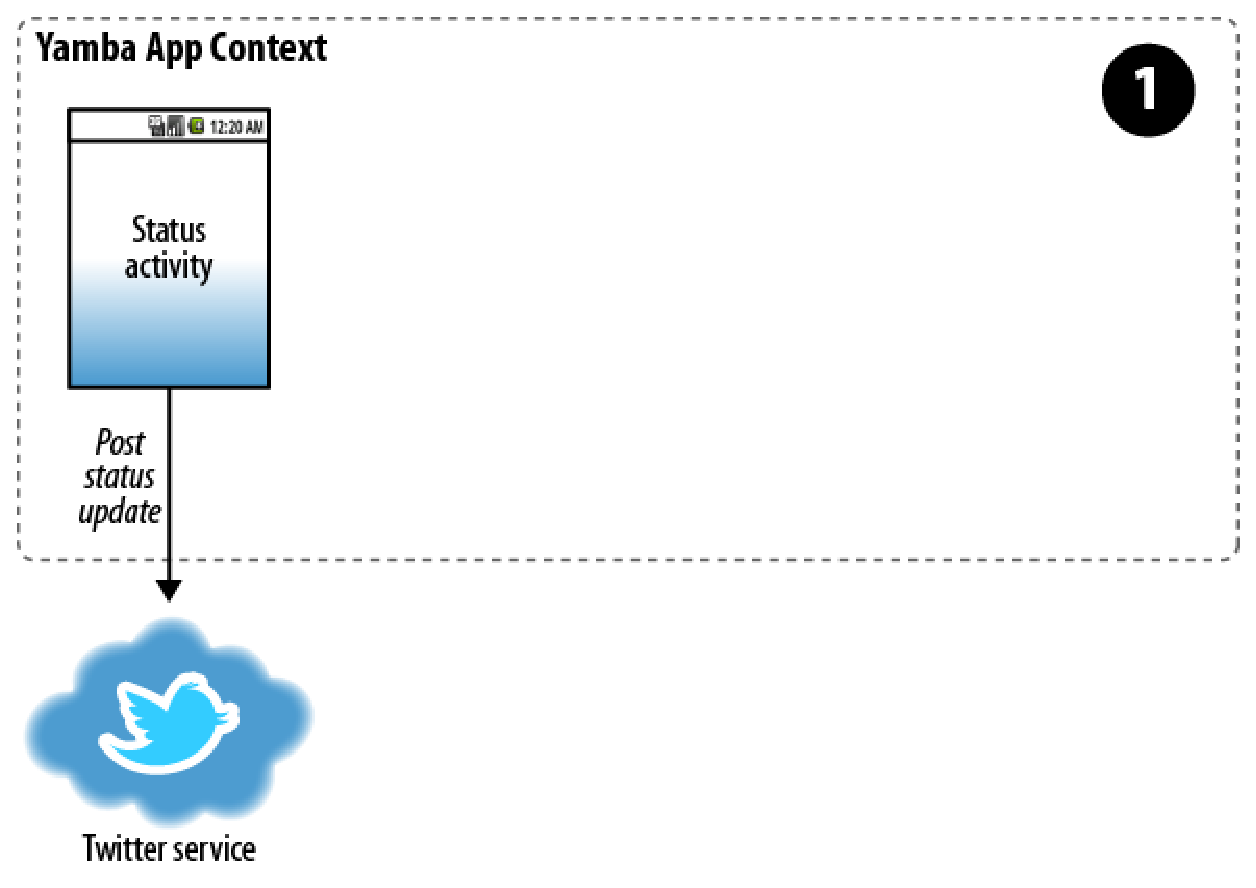
\includegraphics[width=0.65 \textwidth]{fig-64.eps}
\end{frame}
%------------------------------------------------------------------------------
\begin{frame}[fragile]
\frametitle{Git}
Push an existing repository from the command line
\begin{enumerate}
\item \texttt{git remote add origin https://github.com/carmelocuenca/Yamba.git}
\item \texttt{git push -u origin master}
\end{enumerate}
\end{frame}
%------------------------------------------------------------------------------
\begin{frame}[fragile]
\frametitle{Git}
\begin{enumerate}
\item \texttt{git status}
\item \texttt{git commit -a -m ``Color and Graphics''}
\end{enumerate}

\end{frame}
%------------------------------------------------------------------------------



%------------------------------------------------------------------------------
%%%%%%%%%%%%%%%%%%%%%%%%%%%%%%%%%%%%%%%%%%%%%%%%%%%%%%%%%%%%%%%%%%%%%%%%%%%%%%%%%
\section{Preferences, the Filesystem, the Options Menu, and Intents}
%%%%%%%%%%%%%%%%%%%%%%%%%%%%%%%%%%%%%%%%%%%%%%%%%%%%%%%%%%%%%%%%%%%%%%%%%%%%%%%%
\subsection{Preferences}
\begin{frame}
\frametitle{Preferences}
\begin{columns}
\column{0.70\textwidth}
Preferences are user-specific settings for an application. To create preferences for our application, we need to:
\begin{enumerate}
\item Create a Preference resource file called \texttt{prefs.xml}
\item Implement the \texttt{PrefsActivity.java} file that inflates that resource file
\item Register this new activity with the \texttt{AndroidManifest.xml} file
\item Provide a way to start that activity from the rest of the application
\end{enumerate}
\column{0.25 \textwidth}
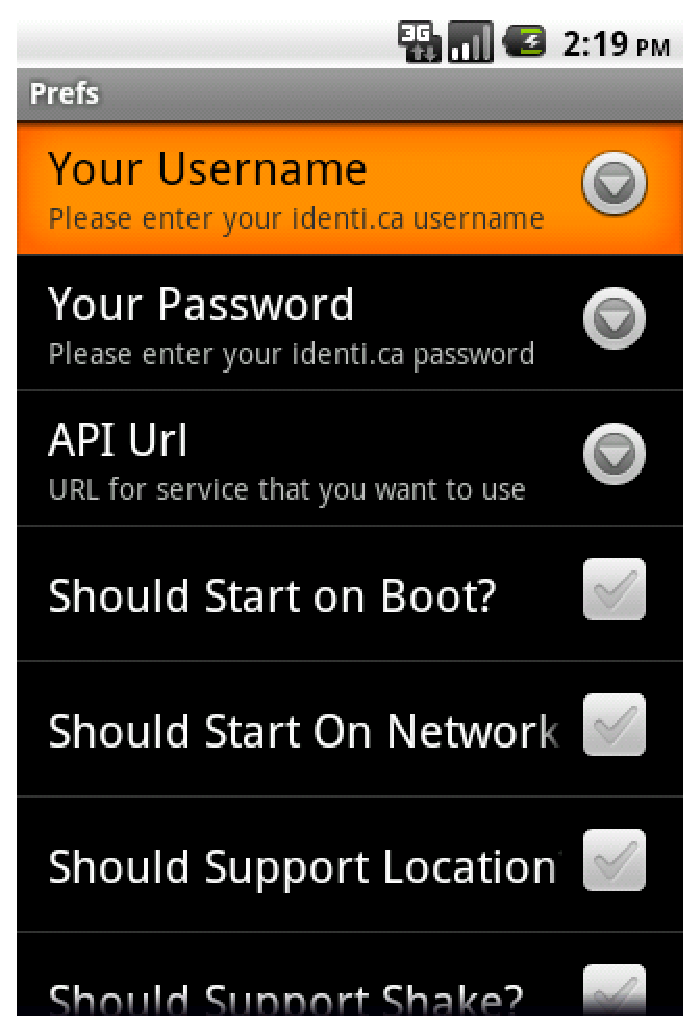
\includegraphics[width= 0.95 \textwidth]{prefrences.eps}
\end{columns}
\end{frame}
%------------------------------------------------------------------------------
\begin{frame}
\frametitle{Prefs Resource}
To start the New Android XML File dialog, go to \texttt{File|New|Android XML File}
\centering
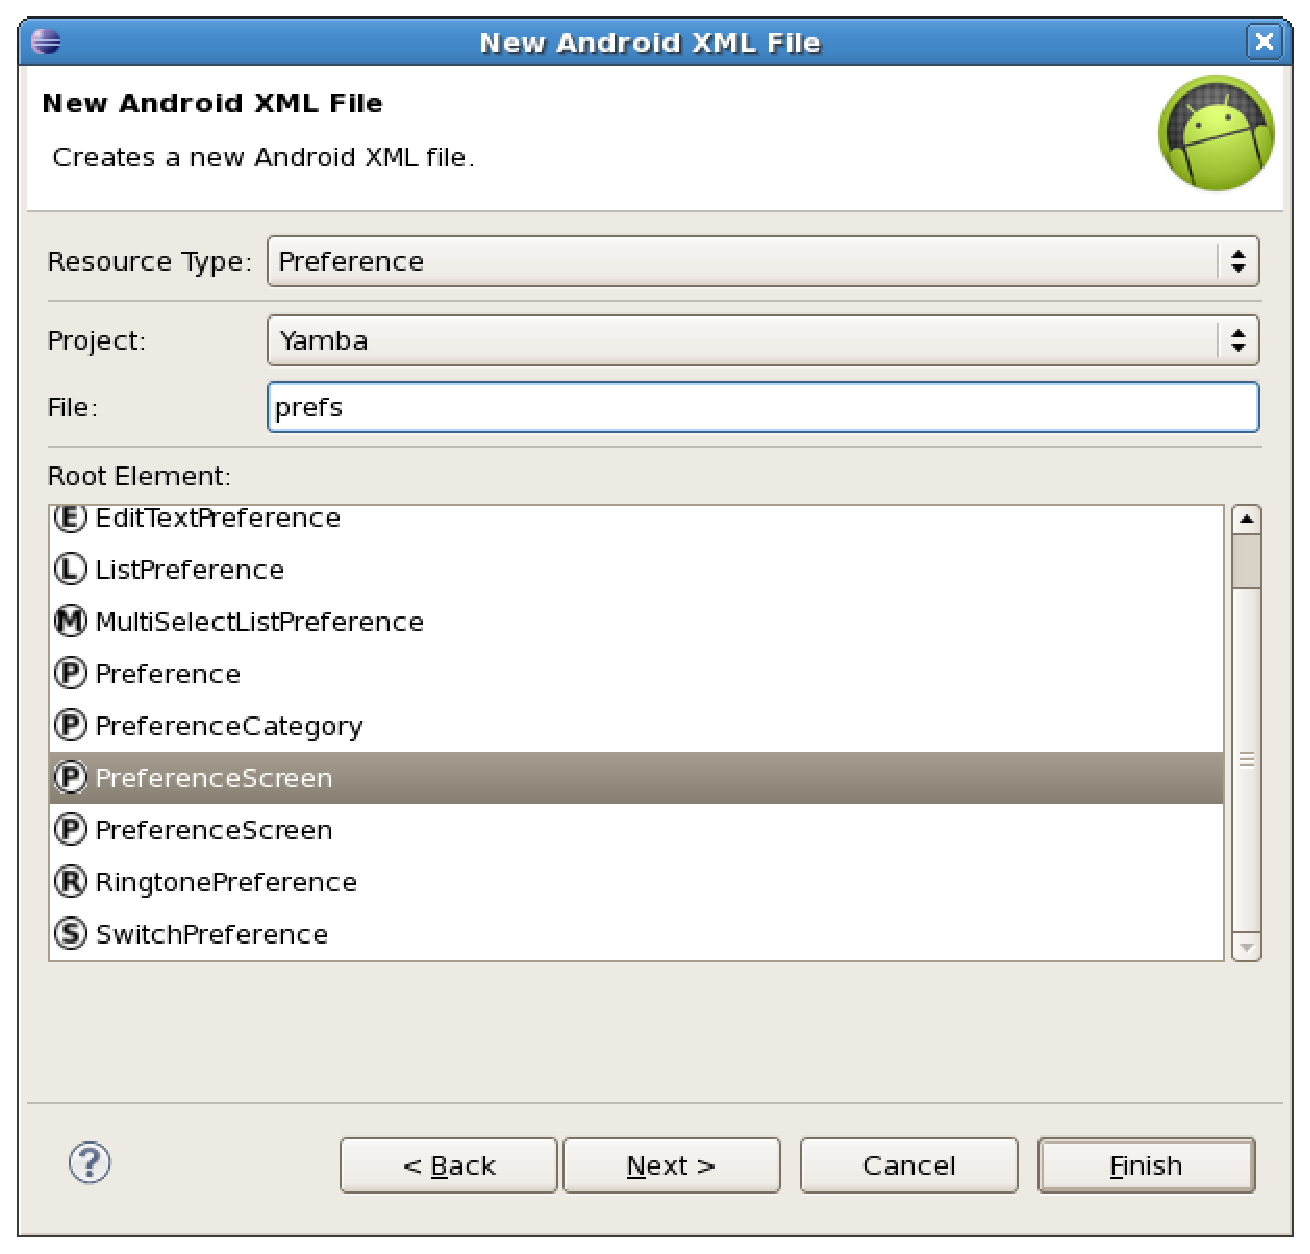
\includegraphics[width= 0.55 \textwidth]{newAndroidXMLFile.eps}
\end{frame}
%------------------------------------------------------------------------------
\begin{frame}
\frametitle{XML Elements}

	\includegraphics[width= 0.80 \textwidth]{xml-elements.eps}

\begin{description}
	\item[Key] A unique identifier for each preference item
	\item[Title] The preference name that the user will see
	\item[Summary] A short description of this preference item
\end{description}
	
\end{frame}
%------------------------------------------------------------------------------
\begin{frame}[containsverbatim]
\frametitle{\texttt{prefs.xml}}
\lstset{language=XML, style=eclipse}
\begin{adjustbox}{width=1.0 \textwidth}
\begin{lstlisting}[caption=res/xml/prefs.xml, basicstyle=\scriptsize,escapechar=$]
<?xml version="1.0" encoding="utf-8"?>
<PreferenceScreen xmlns:android="http://schemas.android.com/apk/res/android" >

    <EditTextPreference
        android:key="username"
        android:summary="@string/summaryUsername"
        android:title="@string/titleUsername" />
    <EditTextPreference
        android:key="password"
        android:summary="@string/summaryPassword"
        android:title="@string/titlePassword" />
    <EditTextPreference
        android:key="apiRoot"
        android:summary="@string/summaryApiRoot"
        android:title="@string/titleApiRoot" />

</PreferenceScreen>
\end{lstlisting}
\end{adjustbox}
\end{frame}
%------------------------------------------------------------------------------
\begin{frame}[containsverbatim]
\frametitle{\texttt{strings.xml}}
\lstset{language=XML, style=eclipse}
\begin{adjustbox}{width=1.0 \textwidth}
\begin{lstlisting}[caption=res/values/strings.xml, basicstyle=\scriptsize,escapechar=$]
<?xml version="1.0" encoding="utf-8"?>
<resources>

    <string name="app_name">Yamba1</string>
    <string name="action_settings">Settings</string>
    <string name="hello_world">Hello world!</string>
    <string name="titleStatus">Status Update</string>
    <string name="hintText">Please enter your 140 character status</string>
    <string name="buttonUpdate">Update</string>
    <string name="tittleUsername">Username</string> <!-- $\circled{1} $-->
    <string name="summaryUsername">Please enter your username</string>
    <string name="tittlePassword">Password</string>
    <string name="summaryPassword">Please enter your password</string>
    <string name="tittleApiRoot">API Root</string>
    <string name="summaryApiRoot">URL API for your service</string>

</resources>
\end{lstlisting}
\end{adjustbox}
\end{frame}
%------------------------------------------------------------------------------
\begin{frame}[containsverbatim]
\frametitle{\texttt{PrefsActivity.java}}
To create an activity, we create a new Java class. In Eclipse, select your package under
your src folder, right-click on the package, and select \texttt{New|Class}.
\lstset{language=java, style=eclipse}
\begin{adjustbox}{width=1.0 \textwidth}
\begin{lstlisting}[caption=src/com.artemisa.yamba/PrefsActivity.java, basicstyle=\scriptsize,escapechar=$]
// .
// .
// .
public class PrefsActivity extends PreferenceActivity { // $\circled{1}$
	@SuppressWarnings("deprecation")
	@Override
	protected void onCreate(Bundle savedInstanceState) { 
		// TODO Auto-generated method stub
		super.onCreate(savedInstanceState);

		$\sout{addPreferencesFromResource}$(R.xml.prefs); // $\circled{2}$
	}
}
\end{lstlisting}
\end{adjustbox}
\end{frame}
%------------------------------------------------------------------------------
\begin{frame}[containsverbatim]
\frametitle{Update the Manifest File}
We have a new \texttt{PrefsActivity} and must add it to the manifest file  \texttt{AndroidManifest.xml}
Choose the Application tab, and then under Application Nodes, choose \texttt{Add|Activity} and name it \texttt{PrefsActivity}

\centering
\includegraphics[width= 0.9 \textwidth]{yamba-manifiest.eps}

\end{frame}
%------------------------------------------------------------------------------
%------------------------------------------------------------------------------
\begin{frame}[containsverbatim]
\frametitle{Update the Manifest File}
\lstset{language=XML, style=eclipse}.
\begin{adjustbox}{width=1.0 \textwidth}
\begin{lstlisting}[caption=YambaManifiest.xml, basicstyle=\scriptsize,escapechar=$]
    <!-- . -->
    <!-- . -->
    <!-- . -->
        <activity
            android:name="com.artemisa.yamba1.StatusActivity"
            android:label="@string/app_name" >
            <intent-filter>
                <action android:name="android.intent.action.MAIN" />

                <category android:name="android.intent.category.LAUNCHER" />
            </intent-filter>
        </activity>

	<activity $\circled{1}$
            android:name="com.artemisa.yamba1.PrefsActivity"
            android:icon="@android:drawable/ic_menu_preferences"
            android:label="@string/tittlePrefs" >
        </activity>
    <!-- . -->
    <!-- . -->
    <!-- . -->
\end{lstlisting}
\end{adjustbox}
\end{frame}
%------------------------------------------------------------------------------
\subsection{The Options Menu}
\begin{frame}
\frametitle{The Options Menu}
The options menu is an Android user interface component that provides standardized
menus to applications. The menus appear at the bottom of the screen when the user
presses the Menu button on the device

To add support for the options menu to an application, we need to do the following:

\begin{enumerate}
\item Edit the \texttt{status.xml} resource where we specify what the menu consists of
\item Edit \texttt{onCreateOptionsMenu()} to the activity that should have this menu. This is
where we inflate the \texttt{status.xml} resource
\item Provide handling of menu events in \texttt{onOptionsItemSelected()}
\end{enumerate}
\end{frame}


%------------------------------------------------------------------------------
\begin{frame}
\frametitle{\texttt{status.xml}}

\centering
\includegraphics[width= 0.8 \textwidth]{menu.eps}
\end{frame}
%------------------------------------------------------------------------------
\begin{frame}[containsverbatim]
\frametitle{Update StatusActivity to Load the Menu}

The first time the Menu button is pressed, the system will call
the activity’s \texttt{onCreateOptionsMenu()} method to inflate the menu from the \texttt{status.xml}
resource

We need to update the \texttt{StatusActivity} to load up the options menu. To do that, edit
the \texttt{onCreateOptionsMenu()} method to \texttt{StatusActivity}

\lstset{language=java, style=eclipse}
\begin{adjustbox}{width=1.0 \textwidth}
\begin{lstlisting}[caption=src/com.artemisa.yamba/StatusActivity.java, basicstyle=\scriptsize,escapechar=$]
// Called first time user clicks on the menu button
@Override
public boolean onCreateOptionsMenu(Menu menu) { // $\circled{1}$
	MenuInflater inflater = getMenuInflater(); 
	inflater.inflate(R.menu.status, menu);
	return true; 
}
\end{lstlisting}
\end{adjustbox}


\end{frame}
%------------------------------------------------------------------------------
\begin{frame}[containsverbatim]
\frametitle{Update StatusActivity to Handle Menu Events}

We also need a way to handle various clicks on the menu items. To do that, we add
another callback method, \texttt{onOptionsItemSelected()}

\lstset{language=java, style=eclipse}
\begin{adjustbox}{width=0.90 \textwidth}
\begin{lstlisting}[caption=src/com.artemisa.yamba/StatusActivity.java, basicstyle=\scriptsize,escapechar=$]
// Called when an options item is clicked
@Override
public boolean onOptionsItemSelected(MenuItem item) {
	switch (item.getItemId()) { //
	case R.id.itemPrefs:
		$\colorbox{light-gray}{startActivity(new Intent(this, PrefsActivity.class));}$// $\circled{1}$
		break;
	}
	return true; //
}

\end{lstlisting}
\end{adjustbox}
\end{frame}
%------------------------------------------------------------------------------
\begin{frame}[containsverbatim]
\frametitle{Shared Preferences}
\begin{itemize}
\item Now that we have a preference activity and a way to save our username, password, and
API root, it is time to make use of it. To programmatically access your preferences, we'll
use the \texttt{SharedPreference} class provided by the Android framework.

\item This class is called \texttt{SharedPreference} because this preference is easily accessible from
any component of this application (activities, services, broadcast receivers, and content
providers)
\end{itemize}
\end{frame}
%------------------------------------------------------------------------------
\begin{frame}[allowframebreaks,containsverbatim]
\frametitle{The StatusActivity Java Class}
\lstset{language=java, style=eclipse, breaklines=true, tabsize=2}
%\begin{adjustbox}{width=1.0 \textwidth}
\centering
\begin{lstlisting}[caption=src/com.artemisa.yamba/StatusActivity.java, basicstyle=\tiny, escapechar=! ]
// .
// .
// .
public class StatusActivity extends Activity implements OnClickListener,
		TextWatcher, OnSharedPreferenceChangeListener { \\ !\circled{1}!

	// .
	// .
	// .
	private TextView textCount;

	private SharedPreferences prefs; !\circled{2}!

	@Override
	protected void onCreate(Bundle savedInstanceState) {
		// .
		// .
		// .
		editText.addTextChangedListener(this);

		// Setup preferences
		prefs = PreferenceManager.getDefaultSharedPreferences(this); // !\circled{3}!
		prefs.registerOnSharedPreferenceChangeListener(this);
	}

	// .
	// .
	// .

	private class PostToTwitter extends AsyncTask<String, Integer, String> {
		@Override
		protected String doInBackground(String... params) {
			// TODO Auto-generated method stub
			try {
				!\colorbox{light-gray}{Twitter.Status status = getTwitter().setStatus(params[0]);}! // !\circled{4}!
				return status.text;

			} catch (TwitterException e) {
				Log.e(TAG, e.toString());
				e.printStackTrace();
				return "Failed to post";
			}
		}

		// .
		// .
		// .
	}
	// .
	// .
	// .
	private Twitter getTwitter() { // !\circled{4}!
		if (twitter == null) { //
			String username, password, apiRoot;
			username = prefs.getString("username", ""); //
			password = prefs.getString("password", "");
			apiRoot = prefs.getString("apiRoot",
					"http://yamba.marakana.com/api");
			// Connect to twitter.com
			twitter = new Twitter(username, password); //
			twitter.setAPIRootUrl(apiRoot); //
		}
		return twitter;
	}

	@Override
	public void onSharedPreferenceChanged(SharedPreferences arg0, String arg1) { // !\circled{5}!
		// TODO Auto-generated method stub
		twitter = null;
	}

}

\end{lstlisting}
%\end{adjustbox}
\end{frame}
%------------------------------------------------------------------------------
\subsection{The Filesystem}
\begin{frame}[containsverbatim]
\frametitle{The Filesystem}
So, where does the device store these preferences? How secure is my username and
password? There are two ways for you to access the filesystem on an Android device: 

\begin{enumerate}
\item Via Eclipse \texttt{Window|Show View|Other\dots|Android|File Explorer}

\item  The command line \texttt{\$ adb shell}
\end{enumerate}

\end{frame}
%------------------------------------------------------------------------------
\begin{frame}[containsverbatim]
\frametitle{Filesystem Partitions}

\begin{itemize}
\item The system partition (\texttt{/system/}). Android operating system is located in the system partition
\item The SDCard partition (\texttt{/sdcard/})
\item The user data partition at (\texttt{/data/})
	\begin{itemize}
		\item \texttt{/data/app}
		\item \texttt{/data/data}
	\end{itemize}
\end{itemize}

\end{frame}
%------------------------------------------------------------------------------

\begin{frame}[containsverbatim]
\frametitle{Filesystem Security}
So, how secure is this? This is a common question posed by security folks. Storing
usernames and passwords in clear text always raises eyebrows
\begin{itemize}
\item Open up your commandline terminal and type
\end{itemize}

\centering{
\begin{adjustbox}{width=0.75 \textwidth}
\begin{lstlisting}[escapechar=!]
# !\textbf{cd}! /data/data/com.artemisa.yamba/shared_prefs
# !\textbf{cat}! com.artemisa.yamba_preferences.xml
<?xml version='1.0' encoding='utf-8' standalone='yes' ?>
<map>
<string name="password">password</string>
<string name="username">student</string>
<string name="apiRoot">http://yamba.marakana.com/api</string>
</map>
#
\end{lstlisting}
\end{adjustbox}}
\end{frame}
%------------------------------------------------------------------------------
\begin{frame}[fragile]
\frametitle{Git}
\begin{enumerate}
\item \texttt{git status}
\item \texttt{git add .}
\item \texttt{git status}
\item \texttt{git commit -a -m ``Preferences''}
\item \texttt{git remote add carmelocuenca https://github.com/carmelocuenca/Yamba.git}
\item \texttt{git push -u carmelocuenca master}
\end{enumerate}

\end{frame}
%------------------------------------------------------------------------------
\begin{frame}[containsverbatim]
\frametitle{Summary}
\centering
\includegraphics[width= 0.75 \textwidth]{fig-077.eps}
\end{frame}
%------------------------------------------------------------------------------





%%%%%%%%%%%%%%%%%%%%%%%%%%%%%%%%%%%%%%%%%%%%%%%%%%%%%%%%%%%%%%%%%%%%%%%%%%%%%%%%
\section{Services}
%%%%%%%%%%%%%%%%%%%%%%%%%%%%%%%%%%%%%%%%%%%%%%%%%%%%%%%%%%%%%%%%%%%%%%%%%%%%%%%%
\begin{frame}
\frametitle{Services}
\begin{itemize}
\item A \alert{service} is simply a piece of code that runs in the background of your application. It doesn’t have a user interface
\item The only states for ``bound'' services are started and stopped (destroyed)
\item The Yamba application needs to create a service to periodically
connect to the cloud and check for new statuses from the user’s friends. This
service will be always on and always running, regardless of whether the user ever starts
\end{itemize}
\end{frame}
%------------------------------------------------------------------------------
\subsection{The Yamba Application Object}
%%%%%%%%%%%%%%%%%%%%%%%%%%%%%%%%%%%%%%%%%%%%%%%%%%%%%%%%%%%%%%%%%%%%%%%%%%%%%%%%
\begin{frame}
\frametitle{The Yamba Application Object}
An \texttt{Application} object represents the common state of your entire application.
We are going to create our own instance of this object and call it \texttt{YambaApplication}. The
steps for creating the \texttt{YambaApplication} class are:
\begin{enumerate}
\item Create the Java class representing \texttt{YambaApplication}
\item Register the new class with the \texttt{AndroidManifest.xml} file
\end{enumerate}
\end{frame}
%------------------------------------------------------------------------------
\begin{frame}[containsverbatim]
\frametitle{The Yamba Application Class}
Create a new Java class in the same package as the rest of our
classes. Call this class \texttt{YambaApplication}, and it will extend the \texttt{Application} base
class from the framework
\lstset{language=java, style=eclipse, breaklines=true, tabsize=2}
\begin{adjustbox}{width=1.0 \textwidth}
\begin{lstlisting}[caption=src/com/artemisa/yamba/YambaApplication.java, basicstyle=\tiny,escapechar=!]
package com/artemisa/yamba;

import android.app.Application;

public class YambaApplication extends Application { // !\circled{1}!

}
\end{lstlisting}
\end{adjustbox}
\end{frame}
%------------------------------------------------------------------------------
\begin{frame}[allowframebreaks,containsverbatim]
\frametitle{\texttt{YambaApplication.java}}
Move common tasks into this base object

\lstset{language=java, style=eclipse, breaklines=true, tabsize=2}
\begin{lstlisting}[caption=src/com/artemisa/yamba/YambaApplication.java, basicstyle=\tiny,escapechar=!]
// .
// .
// .
public class YambaApplication extends Application implements
		OnSharedPreferenceChangeListener { // !\circled{1}!
	private static final String TAG = YambaApplication.class.getSimpleName();
	private Twitter twitter; // !\circled{2}!
	private SharedPreferences prefs;

	@Override
	public void onCreate() { // !\circled{3}!
		// TODO Auto-generated method stub
		super.onCreate();
		prefs = PreferenceManager.getDefaultSharedPreferences(this);
		prefs.registerOnSharedPreferenceChangeListener(this);
		Log.i(TAG, "onCreated");
	}

	@Override
	public void onTerminate() { // !\circled{4}!
		// TODO Auto-generated method stub
		super.onTerminate();
		Log.i(TAG, "onTerminated");
	}

	public synchronized Twitter getTwitter() { // !\circled{5}!
		if (twitter == null) {
			String username, password, apiRoot;
			username = prefs.getString("username", "");
			password = prefs.getString("password", "");
			apiRoot = prefs.getString("apiRoot",
					"http://yamba.marakana.com/api");
			// Connect to twitter.com
			twitter = new Twitter(username, password);
			twitter.setAPIRootUrl(apiRoot);
		}
		return twitter;
	}

	@Override
	public synchronized void onSharedPreferenceChanged(
			SharedPreferences sharedPreferences, String key) { // !\circled{6}!
		// TODO Auto-generated method stub
		Log.d(TAG, "onSharedPreferenceChanged()");
		twitter = null;

	}
}
\end{lstlisting}
\end{frame}
%------------------------------------------------------------------------------
\begin{frame}[containsverbatim]
\frametitle{Update de Manifest File \texttt{AndroidManifest.xml}}
\centering
\includegraphics[width= 0.75 \textwidth]{update-manifest.eps}
\end{frame}
%------------------------------------------------------------------------------
\begin{frame}[allowframebreaks,containsverbatim]
\frametitle{\texttt{AndroidManifest.xml}}
\lstset{language=XML, style=eclipse,breaklines=true,  basicstyle=\tiny,tabsize=2}
\begin{lstlisting}[caption=AndroidManifest.xml, basicstyle=\tiny,escapechar=$]
<?xml version="1.0" encoding="utf-8"?>
    <!-- . -->
    <!-- . -->
    <!-- . -->

    <application
        android:name="YambaApplication" $\circled{1}$
        android:allowBackup="true"
        android:icon="@drawable/ic_launcher"
        android:label="@string/app_name"
        android:theme="@style/AppTheme" >
        <!-- . -->
        <!-- . -->
        <!-- . -->
    </application>

</manifest>
\end{lstlisting}
\end{frame}
%------------------------------------------------------------------------------
\begin{frame}[allowframebreaks,containsverbatim]
\frametitle{The StatusActivity Java Class}
\lstset{language=java, style=eclipse, breaklines=true, tabsize=2}
%\begin{adjustbox}{width=1.0 \textwidth}
\centering
\begin{lstlisting}[caption=src/com/artemisa/yamba/StatusActivity.java, basicstyle=\tiny,, escapechar=! ]
// .
// .
// .
public class StatusActivity extends Activity implements OnClickListener,
		TextWatcher { \\ !\circled{1}!

	// .
	// .
	// .

	private class PostToTwitter extends AsyncTask<String, Integer, String> {
		@Override
		protected String doInBackground(String... params) {
			// TODO Auto-generated method stub
			try {
				Twitter.Status status = ((YambaApplication) getApplication()).getTwitter().setStatus(params[0]); // !\circled{2}!
				return status.text;

			} catch (TwitterException e) {
				Log.e(TAG, e.toString());
				e.printStackTrace();
				return "Failed to post";
			}
		}

		// .
		// .
		// .
	}
	// .
	// .
	// .
	
}

\end{lstlisting}
%\end{adjustbox}
\end{frame}
%------------------------------------------------------------------------------
\begin{frame}[fragile]
\frametitle{Git}
\begin{enumerate}
\item \texttt{git status}
\item \texttt{git add .}
\item \texttt{git status}
\item \texttt{git commit -a -m ``Yamba Application Object''}
\end{enumerate}

\end{frame}
%------------------------------------------------------------------------------
\subsection{Updater Service}
\begin{frame}
\frametitle{Updater Service}
Steps to creating a service are:
\begin{enumerate}
\item Create the Java class representing your service
\item Register the service in the Android manifest file
\item Start the service
\end{enumerate}
\end{frame}
%------------------------------------------------------------------------------
\begin{frame}
\frametitle{Create the Java class \texttt{UpdaterService.java}}
The basic procedure for creating a service, as with activities and other main building
blocks, is to subclass a \texttt{Service} class provided by the Android framework
\begin{columns}
\column{0.45 \textwidth}
\begin{itemize}
\item \texttt{onCreate()} Called when the service is created for the first time
\item \texttt{onStartCommand()} Called when the service is started
\item \texttt{onDestroy()} Called when the service is terminated
\end{itemize}
\column{0.55 \textwidth}
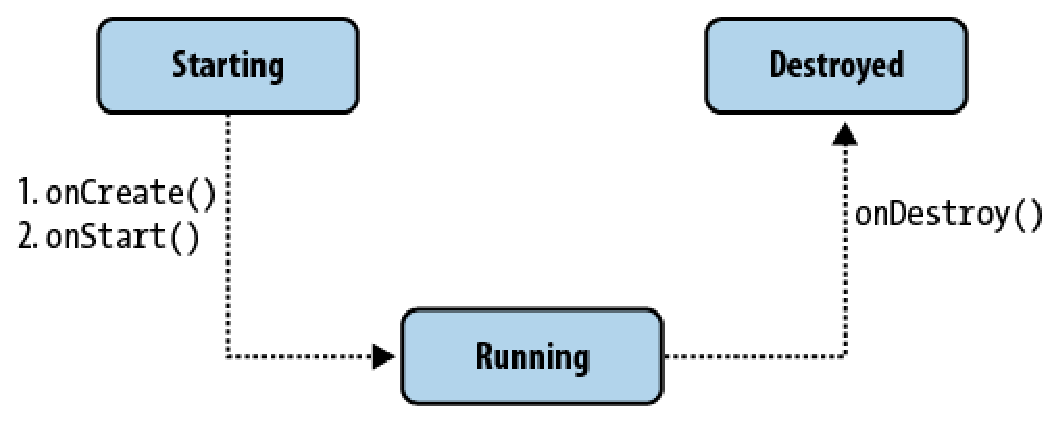
\includegraphics[width= 1.10 \textwidth]{fig-078.eps}
\end{columns}
\end{frame}
%------------------------------------------------------------------------------
\begin{frame}[allowframebreaks,containsverbatim]
\frametitle{\texttt{UpdaterService.java}}
Create the Java class representing \texttt{UpdaterService}

\lstset{language=java, style=eclipse, breaklines=true, tabsize=2}
\begin{lstlisting}[caption=src/com/artemisa/yamba/UpdaterService.java, basicstyle=\tiny,escapechar=!]
// .
// .
// .
public class UpdaterService extends Service {
	static final String TAG = "UpdaterService"; // !\circled{1}!

	@Override
	public IBinder onBind(Intent arg0) { !\circled{2}!
		// TODO Auto-generated method stub
		return null;
	}

	@Override
	public void onCreate() {  // !\circled{3}!
		// TODO Auto-generated method stub
		super.onCreate();
		Log.d(TAG, "onCreated");
	}

	@Override
	public void onDestroy() {  !\circled{4}!
		// TODO Auto-generated method stub
		super.onDestroy();
		Log.d(TAG, "onDestroyed");
	}

	@Override
	public int onStartCommand(Intent intent, int flags, int startId) { !\circled{5}!
		// TODO Auto-generated method stub
		super.onStartCommand(intent, flags, startId);
		Log.d(TAG, "onStarted");
		return START_STICKY;
	}

}
\end{lstlisting}
\end{frame}
%------------------------------------------------------------------------------
\begin{frame}[allowframebreaks,containsverbatim]
\frametitle{Update de Manifest File \texttt{AndroidManifest.xml}}
\lstset{language=XML, style=eclipse,breaklines=true, tabsize=2}
\begin{lstlisting}[caption=AndroidManifest.xml, basicstyle=\tiny,escapechar=$]
<?xml version="1.0" encoding="utf-8"?>
<manifest xmlns:android="http://schemas.android.com/apk/res/android"
    <!-- . -->
    <!-- . -->
    <!-- . -->

        <service android:name="com/artemisa/yamba.UpdaterService" > <!-- $\circled{1}$ -->
        </service>
    </application>

</manifest>
\end{lstlisting}
\end{frame}
%------------------------------------------------------------------------------
\begin{frame}[allowframebreaks,containsverbatim]
\frametitle{Add Menu Items}
We need a way to start and stop the service.
The easiest way would be to add a menu button to our options menu 
\lstset{language=XML, style=eclipse,breaklines=true, tabsize=2}
\begin{lstlisting}[caption=res/menu/status.xml, basicstyle=\tiny,escapechar=$]
<menu xmlns:android="http://schemas.android.com/apk/res/android" >

    <!-- . -->
    <!-- . -->
    <!-- . -->
    <item <!- $\circled{1}$ -->
        android:id="@+id/itemServiceStart"
        android:icon="@android:drawable/ic_media_play"
        android:title="@string/tittleServiceStart">
    </item>
    <item <!- $\circled{2}$ -->
        android:id="@+id/itemServiceStop"
        android:icon="@android:drawable/ic_media_pause"
        android:title="@string/tittleServiceStop">
    </item>

</menu>
\end{lstlisting}
\end{frame}
%------------------------------------------------------------------------------
\begin{frame}[allowframebreaks,containsverbatim]
\frametitle{Update the Options Menu Handling}
\lstset{language=java, style=eclipse, breaklines=true, tabsize=2}
\begin{lstlisting}[caption=src/com/artemisa/yamba/StatusActiviy.java, basicstyle=\tiny,escapechar=!]
// .
// .
// .
// Called when an options item is clicked
@Override
public boolean onOptionsItemSelected(MenuItem item) {
	switch (item.getItemId()) {
	case R.id.itemServiceStart:
		startService(new Intent(this, UpdaterService.class)); // !\circled{1}!
		break;
	case R.id.itemServiceStop:
		stopService(new Intent(this, UpdaterService.class)); //  !\circled{2}!
		break;
	case R.id.itemPrefs:
		startActivity(new Intent(this, PrefsActivity.class));
		break;
	}
	return true;
}
\end{lstlisting}
\end{frame}

%------------------------------------------------------------------------------
\begin{frame}[allowframebreaks,containsverbatim]
\frametitle{Testing the Serivce}
To verify that your service is working
\begin{itemize}
 \item  Open up your LogCat and look for the appropriate
log messages that you generated in your service code
 \item Or press \texttt{Menu} and choose \texttt{Setting|Application|Running services}
\end{itemize}

\end{frame}
%------------------------------------------------------------------------------
\begin{frame}[fragile]
\frametitle{Git}
\begin{enumerate}
\item \texttt{git status}
\item \texttt{git add .}
\item \texttt{git status}
\item \texttt{git commit -a -m ``UpdaterStatus''}
\end{enumerate}

\end{frame}
%------------------------------------------------------------------------------
\begin{frame}[allowframebreaks,containsverbatim]
\frametitle{Looping in the Service}
\begin{itemize}
\item Our service is supposed to wake up every so often, check the online service
for new status updates, an then go back to ``sleep'' for some time
\item A  way to implement this is to have our service run in a loop and pause execution between iterations. Java provides a \texttt{Thread.sleep()}
\item The service could require a good deal of time to make its connection to Twitter and pull in friends’ status data
\end{itemize}


\end{frame}
%------------------------------------------------------------------------------
\begin{frame}[allowframebreaks,containsverbatim]
\frametitle{\texttt{UpdaterService.java}}
\lstset{language=java, style=eclipse, breaklines=true, tabsize=2}
\begin{lstlisting}[caption=src/com/artemisa/yamba/UpdaterService.java, basicstyle=\tiny,escapechar=!]
// .
// .
// .

public class UpdaterService extends Service {
	private static final String TAG = "UpdaterService";
	private static final int DELAY = 60000; // a minute !\circled{1}!
	private boolean runFlag = false; // !\circled{2}!
	private Updater updater;

	@Override
	public IBinder onBind(Intent arg0) {
		// TODO Auto-generated method stub
		return null;
	}

	@Override
	public void onCreate() {
		// TODO Auto-generated method stub
		super.onCreate();

		updater = new Updater(); // !\circled{3}!

		Log.d(TAG, "onCreated");

	}

	@Override
	public void onDestroy() {
		// TODO Auto-generated method stub
		super.onDestroy();

		runFlag = false; // !\circled{4}!
		updater.interrupt(); // !\circled{5}!
		updater = null;

		Log.d(TAG, "onDestroyed");
	}

	@Override
	public int onStartCommand(Intent intent, int flags, int startId) {
		// TODO Auto-generated method stub
		super.onStartCommand(intent, flags, startId);

		runFlag = true; // !\circled{6}!
		updater.start();

		Log.d(TAG, "onStarted"); 
		return START_STICKY;
	}

	/*
	 * Threads tha permos the actual update from the online service
	 */
	private class Updater extends Thread { // !\circled{7}!

		private Updater() {
			super("UpdaterService-Updater"); // !\circled{8}!
			// TODO Auto-generated constructor stub
		}

		@Override
		public void run() { // !\circled{9}!
			UpdaterService updaterService = UpdaterService.this; // !\circled{10}!
			while (updaterService.runFlag) { // !\circled{11}!
				Log.d(TAG, "Updater running");
				try {
					// Some work goes here ...
					Log.d(TAG, "Updater ran");
					Thread.sleep(DELAY); // !\circled{12}!
				} catch (InterruptedException e) { // !\circled{13}!
					updaterService.runFlag = false;
				}
			}
		}

	} // Updater

}

\end{lstlisting}
\end{frame}

%------------------------------------------------------------------------------
\begin{frame}[fragile]
\frametitle{Testing the Service}
\lstset{language=shell}
\begin{lstlisting}[caption=LogCat output]
04-18 14:43:47.925: D/UpdaterService(8858): onCreated
04-18 14:43:47.925: D/UpdaterService(8858): onStarted
04-18 14:43:48.002: D/UpdaterService(8858): Updater running
04-18 14:43:48.002: D/UpdaterService(8858): Updater ran
04-18 14:44:48.005: D/UpdaterService(8858): Updater running
04-18 14:44:48.005: D/UpdaterService(8858): Updater ran
04-18 14:45:48.008: D/UpdaterService(8858): Updater running
04-18 14:45:48.008: D/UpdaterService(8858): Updater ran
04-18 14:46:48.008: D/UpdaterService(8858): Updater running
04-18 14:46:48.008: D/UpdaterService(8858): Updater ran
\end{lstlisting}
\end{frame}
%------------------------------------------------------------------------------


%------------------------------------------------------------------------------
\begin{frame}[fragile]
\frametitle{Git}
\begin{enumerate}
\item \texttt{git status}
\item \texttt{git add .}
\item \texttt{git status}
\item \texttt{git commit -a -m ``Looping in the Service''}
\end{enumerate}

\end{frame}
%------------------------------------------------------------------------------
\begin{frame}[fragile]
\frametitle{Pulling Data from Twitter}
The \texttt{jtwitter.jar} library exposes most of them to us via the \texttt{Twitter} class. Perhaps one
of the most appropriate methods is \texttt{getFriendsTimeline()}, which returns the 20 most
recent posts made over the past 24 hours from the user and her friends
\end{frame}
%------------------------------------------------------------------------------
\begin{frame}[allowframebreaks,containsverbatim]
\frametitle{\texttt{UpdaterService.java}}
\lstset{language=java, style=eclipse, breaklines=true, tabsize=2}
\begin{lstlisting}[caption=src/com/artemisa/yamba/UpdaterService.java, basicstyle=\tiny,escapechar=!]
// .
// .
// .
	/*
	 * Threads tha permos the actual update from the online service
	 */
	private class Updater extends Thread {
		List<Twitter.Status> timeline; // !\circled{1}!

		private Updater() {
			super("UpdaterService-Updater");
			// TODO Auto-generated constructor stub
		}

		@Override
		public void run() {
			UpdaterService updaterService = UpdaterService.this;
			while (updaterService.runFlag) {
				Log.d(TAG, "Updater running");
				try {
					try {
						// Get the timeline from the cloud
						timeline = ((YambaApplication) getApplication()).getTwitter().getFriendsTimeline(); !\circled{2}!
					} catch (TwitterException e) {
						Log.e(TAG, "Failed to connect to twitter service", e); !\circled{3}!
					}
					// Loop over the timeline and print it out
					for (Twitter.Status status : timeline) { // !\circled{4}!
						Log.d(TAG, String.format("%s: %s", status.user.name,
								status.text)); // !\circled{5}!
					}
					Log.d(TAG, "Updater ran");
					Thread.sleep(DELAY);
				} catch (InterruptedException e) {
					updaterService.runFlag = false;
				}
			}
		}

	}

}

\end{lstlisting}
\end{frame}

%------------------------------------------------------------------------------
\begin{frame}[fragile]
\frametitle{Git}
\begin{enumerate}
\item \texttt{git status}
\item \texttt{git add .}
\item \texttt{git status}
\item \texttt{git commit -a -m ``Pulling Data from Twitter''}
\item \texttt{git remote add carmelocuenca https://github.com/carmelocuenca/Yamba.git}
\item \texttt{git push -u carmelocuenca master}
\end{enumerate}

\end{frame}
%------------------------------------------------------------------------------

%%%%%%%%%%%%%%%%%%%%%%%%%%%%%%%%%%%%%%%%%%%%%%%%%%%%%%%%%%%%%%%%%%%%%%%%%%%%%%%%
\section{The Database}
%%%%%%%%%%%%%%%%%%%%%%%%%%%%%%%%%%%%%%%%%%%%%%%%%%%%%%%%%%%%%%%%%%%%%%%%%%%%%%%%
\begin{frame}
\frametitle{The Database}
\texttt{SQLite} is an open source database that has been around for a long time, is quite stable
\begin{itemize}
\item It’s a zero-configuration database
\item It doesn’t have a server. It is basically
a set of libraries that provide the database functionality
\item It’s a single-file database
\item It’s open source
\end{itemize}
\end{frame}
%------------------------------------------------------------------------------
\begin{frame}
\frametitle{\texttt{DbHelper}}
Android provides an elegant interface for your app to interact with an SQLite database
\begin{enumerate}
\item To access the database, you first need a helper class that provides a ``connection'' to
the database, creating the connection if it doesn’t already exist. This class, provided to
you by the Android framework, is called \alert{\texttt{SQLiteOpenHelper}}
\item The database class it returns is an instance of \alert{\texttt{SQLiteDatabase}}
\end{enumerate}

DbHelper offers (CRUD: create, read (query), update, and delete):
\begin{description}
\item [\texttt{insert()}] Inserts one or more rows into the database
\item [\texttt{query()}] Requests rows matching the criteria you specify
\item [\texttt{update()}] Replaces ones or more rows that match the criteria you specify
\item [\texttt{delete()}] Deletes rows matching the criteria you specify
\end{description}
\end{frame}
%------------------------------------------------------------------------------
\begin{frame}
\frametitle{\texttt{First Example}}
Create a new Java class in the same package as the rest of our
classes. Call this class \texttt{DBHelper}, and it will extend the \texttt{SQLiteOpenHelper} base
class from the framework. We then need to implement ;
\begin{itemize}
\item The class’s constructor
\item  \texttt{public abstract void onCreate (SQLiteDatabase db)}\\Called when the database is created for the first time. This is where the creation of tables and the initial population of the tables should happen
\item \texttt{public abstract void onUpgrade (SQLiteDatabase db, int oldVersion, int newVersion)}\\ Called when the database needs to be upgraded. The implementation should use this method to drop tables, add tables \dots
\end{itemize}

\end{frame}
%------------------------------------------------------------------------------
\begin{frame}[allowframebreaks,containsverbatim]
\frametitle{\texttt{DBHelper.java}}

\lstset{language=java, style=eclipse, breaklines=true, tabsize=2}
\begin{lstlisting}[caption=src/com/artemisa/yamba/DBHelper.java, basicstyle=\tiny,escapechar=$]
// .
// .
// .

public class DBHelper extends SQLiteOpenHelper { //  $\circled{1}$

	static final String TAG = DBHelper.class.getSimpleName();
	static final String DB_NAME = "timeline.db"; //  $\circled{2}$
	static final int DB_VERSION = 1; //
	static final String TABLE = "timeline";
	static final String C_ID = "id";
	static final String C_CREATED_AT = "created_at";
	static final String C_SOURCE = "source";
	static final String C_TEXT = "txt";
	static final String C_USER = "user";

	public DBHelper(Context context) { //  $\circled{3}$
		// TODO Auto-generated constructor stub

		super(context, DB_NAME, null, DB_VERSION);
	}

	// Called only once, first time the DB is created
	@Override
	public void onCreate(SQLiteDatabase db) { //  $\circled{4}$
		// TODO Auto-generated method stub
		String sql = "create table" + TABLE + " (" + C_ID
				+ " int primary key, " + C_CREATED_AT + " int, " + C_SOURCE + " text, " + C_USER
				+ " text, " + C_TEXT + " text)";
		db.execSQL(sql);
		Log.d(TAG, "onCreated sql:" + sql);
	}

	// Called whenever newVersion != to oldVersion
	@Override
	public void onUpgrade(SQLiteDatabase db, int oldVersion, int newVersion) { //  $\circled{5}$
		// TODO Auto-generated method stub
		// Typically do ALTER TABLE statements, but...we're just in development,
		// so:
		db.execSQL("drop table if exists " + TABLE); // drops the old database
		Log.d(TAG, "onUpdated");
		onCreate(db); // run onCreate to get new database
	}

}

\end{lstlisting}
\end{frame}
%------------------------------------------------------------------------------
%------------------------------------------------------------------------------
\begin{frame}[allowframebreaks,containsverbatim]
\frametitle{\texttt{Update UpdaterService}}

\lstset{language=java, style=eclipse, breaklines=true, tabsize=2}
\begin{lstlisting}[caption=src/com/artemisa/yamba/UpdaterService.java, basicstyle=\tiny,escapechar= $]
// .
// .
// .

public class UpdaterService extends Service {
	private static final String TAG = "UpdaterService";
	private static final int DELAY = 60000; // a minute
	private boolean runFlag = false;
	private Updater updater;
	private YambaApplication yamba; // $\circled{1}$
	private DBHelper dbHelper; // $\circled{2}$

	@Override
	public IBinder onBind(Intent arg0) {
		// TODO Auto-generated method stub
		return null;
	}

	@Override
	public void onCreate() {
		// TODO Auto-generated method stub
		super.onCreate();
		yamba = (YambaApplication) getApplication(); $\circled{3}$
		dbHelper = new DBHelper(yamba); $\circled{4}$
		updater = new Updater();

		Log.d(TAG, "onCreated");

	}

	// .
	// .
	// .

	/*
	 * Threads tha permos the actual update from the online service
	 */
	private class Updater extends Thread {
		List<Twitter.Status> timeline;

		private Updater() {
			super("UpdaterService-Updater");
			// TODO Auto-generated constructor stub
		}

		@Override
		public void run() {
			UpdaterService updaterService = UpdaterService.this;
			while (updaterService.runFlag) {
				Log.d(TAG, "Updater running");
				try {
					try {
						// Get the timeline from the cloud
						timeline = updaterService.yamba.getTwitter() 
								.getFriendsTimeline(); // $\circled{4}$  
					} catch (TwitterException e) {
						Log.e(TAG, "Failed to connect to twitter service", e);
					}

					// Open the database for writing
					SQLiteDatabase db = dbHelper.getWritableDatabase(); // $\circled{5}$

					// Loop over the timeline and print it out
					ContentValues values = new ContentValues(); // $\circled{6}$
					for (Twitter.Status status : timeline) { // $\circled{7}$
						// Insert into database
						values.clear(); // $\circled{8}$
						values.put(DBHelper.C_ID, status.id);
						values.put(DBHelper.C_CREATED_AT,
								status.createdAt.getTime());
						values.put(DBHelper.C_SOURCE, status.source);
						values.put(DBHelper.C_TEXT, status.text);
						values.put(DBHelper.C_USER, status.user.name);
						try {
							db.insertOrThrow(DBHelper.TABLE, null, values); // $\circled{9}$
							Log.d(TAG, String.format("%s: %s",
									status.user.name, status.text));
						} catch (SQLException e) {
							// TODO Auto-generated catch block
							Log.e(TAG, e.toString());
							e.printStackTrace();
						}

					}
					db.close(); // $\circled{10}$

					Log.d(TAG, "Updater ran");
					Thread.sleep(DELAY);
				} catch (InterruptedException e) {
					updaterService.runFlag = false;
				}
			}
		}

	}

}

\end{lstlisting}
\end{frame}
%------------------------------------------------------------------------------
\begin{frame}
\frametitle{Testing the service}
To see whether your database schema was created properly:
\begin{itemize}
\item Open up your terminal or command-line window
\item Type \texttt{adb shell} to connect to your running emulator or physical phone
\item Change the directory to the location of your database file by typing \texttt{cd /data/data/com.artemisa.yamba/databases/}
\item Connect to the database with the \texttt{sqlite3 timeline.db} command. At this point, you can send commands to your SQLite database:
\begin{itemize}
\item \texttt{sqlite> .schema;}
\item \texttt{sqlite> SELECT * FROM timeline;}
\end{itemize}
\end{itemize}

\end{frame}
%------------------------------------------------------------------------------
\begin{frame}[fragile]
\frametitle{Git}
\begin{enumerate}
\item \texttt{git status}
\item \texttt{git add .}
\item \texttt{git status}
\item \texttt{git commit -a -m ``Database''}
\end{enumerate}

\end{frame}
%------------------------------------------------------------------------------
\begin{frame}[fragile]
\frametitle{Refactoring Status Data}
The work we did previously for the \texttt{UpdaterService} is not ideal for supporting our next
user of this data: the \texttt{TimelineActivity}. Since \texttt{TimelineActivity} will also need to access
the same database and fetch the same data, it would be better if we would share some
of the same functionality between the \texttt{UpdaterService} and the \texttt{TimelineActivity}.
In order to do that, we’ll create a new Java class, \texttt{StatusData}, and make it the common
container for database-related functionality . It will be hiding (encapsulating)
SQLite in a higher-level class accessible to other parts of the Yamba application.
The rest of our app will then just ask for \texttt{StatusData}
\end{frame}
%------------------------------------------------------------------------------
\begin{frame}[allowframebreaks,containsverbatim]
\frametitle{\texttt{StatusData.java}}
\lstset{language=java, style=eclipse, breaklines=true, tabsize=2}
\begin{lstlisting}[caption=src/com/artemisa/yamba/StatusData.java, basicstyle=\tiny,escapechar= $]
// .
// .
// .
public class StatusData {
	static final String TAG = StatusData.class.getSimpleName();
	static final String DB_NAME = "timeline.db";
	static final int DB_VERSION = 1; //
	static final String TABLE = "timeline";
	static final String C_ID = "id";
	static final String C_CREATED_AT = "created_at";
	static final String C_SOURCE = "source";
	static final String C_TEXT = "txt";
	static final String C_USER = "user";

	private static final String[] MAX_CREATED_AT_COLUMNS = { "max("
			+ StatusData.C_CREATED_AT + ")" }; // $\circled{1}$

	public class DBHelper extends SQLiteOpenHelper { // $\circled{2}$

		public DBHelper(Context context) {
			// TODO Auto-generated constructor stub

			super(context, DB_NAME, null, DB_VERSION);
		}

		// Called only once, first time the DB is created
		@Override
		public void onCreate(SQLiteDatabase db) {
			// TODO Auto-generated method stub
			String sql = "create table " + TABLE + " (" + C_ID
					+ " int primary key, " + C_CREATED_AT + " int, " + C_SOURCE
					+ " text, " + C_USER + " text, " + C_TEXT + " text)";
			db.execSQL(sql);
			Log.d(TAG, "onCreated sql:" + sql);
		}

		// Called whenever newVersion != to oldVersion
		@Override
		public void onUpgrade(SQLiteDatabase db, int oldVersion, int newVersion) {
			// TODO Auto-generated method stub
			// Typically do ALTER TABLE statements, but...we're just in
			// development,
			// so:
			db.execSQL("drop table if exists " + TABLE); // drops the old database
			Log.d(TAG, "onUpdated");
			onCreate(db); // run onCreate to get new database
		}
	}

	private DBHelper dbHelper; // $\circled{3}$

	public StatusData(Context context) { // $\circled{4}$
		dbHelper = new DBHelper(context);
		Log.i(TAG, "Initialized data");
	}

	public void close() {
		dbHelper.close();
	}

	public void insertOrIgnore(ContentValues values) { // $\circled{5}$
		Log.d(TAG, "insertOrIgnore" + values);
		// Open the database for writing
		SQLiteDatabase db = dbHelper.getWritableDatabase();

		try {
			db.insertWithOnConflict(StatusData.TABLE, null, values,
					SQLiteDatabase.CONFLICT_IGNORE);
		} finally {
			db.close();
		}
	}

	/**
	 * 
	 * @return Timestamp of the latest status we ahve it the database
	 */
	public long getLatestStatusCreatedAtTime() { // $\circled{6}$
		SQLiteDatabase db = this.dbHelper.getReadableDatabase();
		try {
			Cursor cursor = db.query(TABLE, MAX_CREATED_AT_COLUMNS, null, null,
					null, null, null);
			try {
				return cursor.moveToNext() ? cursor.getLong(0) : Long.MIN_VALUE;
			} finally {
				cursor.close();
			}
		} finally {
			db.close();
		}
	}

}

\end{lstlisting}
\end{frame}
%------------------------------------------------------------------------------
%------------------------------------------------------------------------------
\begin{frame}[allowframebreaks,containsverbatim]
\frametitle{\texttt{YambaApplication.java}}

\lstset{language=java, style=eclipse, breaklines=true, tabsize=2}
\begin{lstlisting}[caption=src/com/artemisa/yamba/YambaApplication.java, basicstyle=\tiny,escapechar= $]
// .
// .
// .
public class YambaApplication extends Application implements
		OnSharedPreferenceChangeListener {
	private static final String TAG = YambaApplication.class.getSimpleName();
	private Twitter twitter;
	private SharedPreferences prefs;

	private StatusData statusData; // $\circled{1}$

	public StatusData getStatusData() { // $\circled{2}$
		return statusData;
	}

	@Override
	public void onCreate() {
		// TODO Auto-generated method stub
		super.onCreate();

		prefs = PreferenceManager.getDefaultSharedPreferences(this);
		prefs.registerOnSharedPreferenceChangeListener(this);

		statusData = new StatusData(this); // $\circled{3}$
		Log.i(TAG, "onCreated");
	}

	// Connects to the online service and puts the latest statuses into DB.
	// Returns the count of new statuses
	public synchronized int fetchStatusUpdates() { // $\circled{4}$
		Log.d(TAG, "Fetching status updates");
		try {
			List<Status> statusUpdates = getTwitter().getFriendsTimeline();
			long latestStatusCreatedAtTime = this.getStatusData()
					.getLatestStatusCreatedAtTime();
			int count = 0;
			ContentValues values = new ContentValues();
			for (Status status : statusUpdates) {
				values.put(StatusData.C_ID, status.getId());
				long createdAt = status.getCreatedAt().getTime();
				values.put(StatusData.C_CREATED_AT, createdAt);
				values.put(StatusData.C_TEXT, status.getText());
				values.put(StatusData.C_USER, status.getUser().getName());
				Log.d(TAG, "Got update with id " + status.getId() + ". Saving");
				this.getStatusData().insertOrIgnore(values);
				if (latestStatusCreatedAtTime < createdAt) {
					count++;
				}
			}
			Log.d(TAG, count > 0 ? "Got " + count + " status updates"
					: "No new status updates");
			return count;
		} catch (RuntimeException e) {
			Log.e(TAG, "Failed to fetch status updates", e);
			return 0;
		}
	}


	// .
	// .
	// .

}

\end{lstlisting}
\end{frame}
%------------------------------------------------------------------------------
%------------------------------------------------------------------------------
\begin{frame}[allowframebreaks,containsverbatim]
\frametitle{\texttt{UpdaterService.java}}

\lstset{language=java, style=eclipse, breaklines=true, tabsize=2}
\begin{lstlisting}[caption=src/com/artemisa/yamba/UpdaterService.java, basicstyle=\tiny,escapechar= $]
// .
// .
// .
public class UpdaterService extends Service {
	// .
	// .
	// .

	/*
	 * Threads tha permos the actual update from the online service
	 */
	private class Updater extends Thread { 

		private Updater() {
			super("UpdaterService-Updater");
			// TODO Auto-generated constructor stub
		}

		@Override
		public void run() {
			UpdaterService updaterService = UpdaterService.this;
			while (updaterService.runFlag) {
				Log.d(TAG, "Updater running");
				try {
					try {
						// Get the timeline from the cloud
						YambaApplication yamba = (YambaApplication) updaterService.getApplication(); // $\circle{1}$
						int newUpdates = yamba.fetchStatusUpdates(); // $\circle{2}$
						if (newUpdates>0){ // $\circle{1}$
							Log.d(TAG, "We have a new status");
						}
						Thread.sleep(DELAY);
					} catch (TwitterException e) {
						Log.e(TAG, "Failed to connect to twitter service", e);
					}

					
				} catch (InterruptedException e) {
					updaterService.runFlag = false;
				}
			}
		}

	}

}


\end{lstlisting}
\end{frame}
%------------------------------------------------------------------------------
\begin{frame}[containsverbatim]
\frametitle{Summary}

\begin{center}
\includegraphics[width= 0.40 \textwidth]{database.eps}
\end{center}



\end{frame}
%------------------------------------------------------------------------------

\begin{frame}[fragile]
\frametitle{Git}
\begin{enumerate}
\item \texttt{git status}
\item \texttt{git add .}
\item \texttt{git status}
\item \texttt{git commit -a -m ``Database with StatusData''}
\item \texttt{git push -u carmelocuenca master}
\end{enumerate}

\end{frame}
%------------------------------------------------------------------------------

\comment{
\section{List and Adapters}

\section{Broadcast Receeivers}

\section{Content Providers}

\section{System Services}

\section{The Android Interface Definition Language}
}

\begin{frame}
\frametitle{Start Up }
\begin{enumerate}
\item Gitttwitter
\begin{enumerate}
\item \texttt{git clone git://github.com/carmelocuenca/Yamba.git}
\item \texttt{git log --pretty=oneline}
\item \texttt{git reset --hard d9938feab266bc4cbef4c4c8b4fa2541be000e87} OnClickListner Commit
\end{enumerate}
\item Starting the Yamba Project. \texttt{File|New Project|Other\dots|Android Application Project}\dots
\item Copy all files \dots from repository to workspace
\item Don't forget \texttt{.gitignore} \texttt{.git} to \texttt{workspace/Yamba}
\end{enumerate}
\end{frame}


\end{document}
